% REMEMBER: You must not plagiarise anything in your report. Be extremely careful.

\documentclass{l4proj}

    
%
% put any additional packages here
%

\begin{document}

%==============================================================================
%% METADATA
\title{Social Acceptability of Novel Interaction Techniques}
\author{Robert B. Thomson}
\date{November 03, 2020}

\maketitle

%==============================================================================
%% ABSTRACT
\begin{abstract}
    Every abstract follows a similar pattern. Motivate; set aims; describe work; explain results.
    \vskip 0.5em
    ``XYZ is bad. This project investigated ABC to determine if it was better. 
    ABC used XXX and YYY to implement ZZZ. This is particularly interesting as XXX and YYY have
    never been used together. It was found that  
    ABC was 20\% better than XYZ, though it caused rabies in half of subjects.''
\end{abstract}

%==============================================================================

% EDUCATION REUSE CONSENT FORM
% If you consent to your project being shown to future students for educational purposes
% then insert your name and the date below to  sign the education use form that appears in the front of the document. 
% You must explicitly give consent if you wish to do so.
% If you sign, your project may be included in the Hall of Fame if it scores particularly highly.
%
% Please note that you are under no obligation to sign 
% this declaration, but doing so would help future students.
%
\def\consentname {Robert Borland Thomson} % your full name
\def\consentdate {02 April 2021} % the date you agree
%
\educationalconsent

%==============================================================================
\tableofcontents
%==============================================================================
%% Notes on formatting
%==============================================================================
% The first page, abstract and table of contents are numbered using Roman numerals and are not
% included in the page count. 
%
% From now on pages are numbered
% using Arabic numerals. Therefore, immediately after the first call to \chapter we need the call
% \pagenumbering{arabic} and this should be called once only in the document. 
%
% Do not alter the bibliography style.
%
% The first Chapter should then be on page 1. You are allowed 40 pages for a 40 credit project and 30 pages for a 
% 20 credit report. This includes everything numbered in Arabic numerals (excluding front matter) up
% to but excluding the appendices and bibliography.
%
% You must not alter text size (it is currently 10pt) or alter margins or spacing.
%
% 
%==================================================================================================================================
%
% IMPORTANT
% The chapter headings here are **suggestions**. You don't have to follow this model if
% it doesn't fit your project. Every project should have an introduction and conclusion,
% however. 
%
%==================================================================================================================================
\chapter{Introduction}

% reset page numbering. Don't remove this!
\pagenumbering{arabic}


\section{Overview}
Social acceptability plays an important role in a person's willingness to use and interact with technology \citep{rico_usable_2010}. Novel interaction modalities and new interactive devices may initially be perceived as socially unacceptable due to being unfamiliar and maybe even unusual to onlookers---especially if it is not clear that a person is using a computing device. The aim of this dissertation is to evaluate the social acceptability of novel interaction techniques for mobile devices, focusing on the use of gestures for input. Device motion gestures (e.g., shaking a phone) and contactless gestures (e.g., waving above the screen) are widely supported by modern smartphones, but are yet to be widely adopted by users, especially contactless gestures.

This work also investigates a new aspect of perceived social acceptability, looking at the relationship between social acceptability and perceptions of how \textit{useful} an interaction may be to a user. Perceived usefulness or benefit to a user could influence perceptions of social acceptability by attributing a clear reason for \textit{why} a person is interacting with a device in a certain way. How this usefulness changes with exposure and familiarity will also be explored (e.g., to see if interactions become more acceptable as users begin to recognise their benefits).

The research begins with a preliminary survey to investigate current opinions on the use of novel interaction techniques and devices. Following this, an Android media player, with incorporated gesture input, was created. User evaluations over the course of one week were used to analyse the effect of using the novel interaction for the purpose of musical enjoyment over a period of time. Observations are made..... And conclusions are drawn.....


\section{Motivation}
Technological advances mean people are interacting in more ways with an increasing number of devices on a daily basis. In turn, people become more and more reliant on new devices and interaction modalities, because they offer more convenient ways of accessing services and information. They can be very efficient at helping us complete tasks in our everyday lives. 

People can often feel that using novel interaction techniques is socially unacceptable (i.e., that their use would be perceived negatively by other people). This is a serious issue for interaction designers and device manufacturers, as negative perceptions may slow down or prevent the adoption of new technologies. If an interaction is not deemed socially acceptable or does not adhere to social norms, the product seems likely to fail. Very few people will be happy to use it in their day to day lives if it might attract unwanted attention or negative perceptions from others.  It is often just taken for granted that if interaction is too different from the current technologies, or has an unclear use case, then the population will not get behind it. For example, Google Glass was negatively affected by lack of acceptance due to perceived privacy concerns, because interactions with the system and its intended applications were unclear.

Social acceptability is largely affected by the location of use and the `audience' of an interaction \citep{rico_usable_2010}. This is likely the case for certain circumstances of interactions. However, I believe that a persons familiarity with an interaction method will have just as large an impact, if not more, than these factors on their perceptions of acceptability. I believe the perceived use of an interaction technique will grow over time. As a result, the user may be more likely to perceive it to be socially acceptable. Possible factors of how quickly and likely these changes to perception are to occur are (1)~how useful a technique is and (2)~how little effort is required to use it, in comparison to the standard method of completing the desired task. These factors will be explored through this work.

\section{Aims}

This project aims to investigate the relationship between effort required, perceived usefulness and social acceptability of novel interaction techniques. It will do this through multiple approaches. First, a survey will investigate views on social norms and stigmas around effort and usefulness. It will investigate how perceived usefulness affects how people currently use or view novel interaction techniques. In particular, it will ask about gesture input, smart glasses and voice assistant interactions, as these technologies have varying levels of social acceptance currently.

After this, a media player will be implemented with integrated motion gesture input for interaction. Evaluation participants will be asked to use the mobile app over the course of a week and will be interviewed at various stages. This longitudinal study aims to see if users become familiar with the method of interaction over the evaluation time period. It is hypothesised that participants will find the gesture interactions more useful and easier to use over time, and in turn it will be perceived to be socially acceptable to use in more situations. It is believed that this work will provide researchers with a new outlook on social acceptability: that the context of a situation is the boundary that must be met socially, but that acceptability is also affected by the user's perceived usefulness and familiarity with an interaction method.

If this belief is confirmed, it is hoped that interaction designers will be able to use the findings to create interaction techniques that scaffold a user's perceptions early on, e.g., by being easy to familiarise ones self with and recognise the utility of, as opposed to being completely socially acceptable ``out of the box''. 


%==================================================================================================================================
\chapter{Related Work}
\section{Overview}

This overview of related research begins with a brief look at novel interaction techniques and their social acceptability. It then explores social norms around usefulness and effort, to understand how these phenomena affect perceptions and behaviour.

\section{Novel Interactions}

In simple terms, an interaction with a device can be described as and action in which a users communicates input to the device, when the device provides output to the user or a combination of both through interfaces. In the field of Human Computer Interaction it is taken to be more of the way one experiences using the device and their perception of it \citep{beaudouin-lafon_designing_2004}. These interactions can use various techniques and are said to be novel when they are not commonly used or new to the users of the devices. These interactions can be through various parts of the device or completely encompass the device itself. 

Various pieces of literature have set guidelines for how interfaces and interactions should be designed \citep{beaudouin-lafon_designing_2004, gong_guidelines_nodate}. However, guidelines and practices change very regularly. There has always been an attention on invisible interfaces for personal use \citep{schiphorst_really_2007}. These prospects will be built on to understand how the effort required to interact dictates the invisibility and if this invisibility relates to how users feel others will perceive them in social situations.

\section{Social Acceptability}

Individuals make decisions on the social acceptability of their actions on a daily basis \citep{pohl_focused_2013}. They do this by using their existing knowledge to assess their surroundings and consider if an action would be deemed acceptable \citep{naegele_presentation_1956}. This is also the case when interacting with technology. Users evaluate their motivations and desire to use a particular technology and weigh this up against social factors and norms, to decide if an action is socially acceptable in the current usage context \citep{rico_usable_2010}; if not (e.g., due to concern it would look strange or attract unwanted attention) then users will not perform that interaction, or will fall back to an alternative modality. This is important for interaction and product designers because if a product or interaction technique is perceived to be socially unacceptable, users will not be willing to use them and adoption will be limited.

There are some widely given structures of how social acceptability of a device can be assessed. These will be considered in this work, although a slightly different approach will be taken as this project aims to investigate other factors that might affect acceptability. \citet{rico_usable_2010} suggested that users see the interaction as a performance that must be done appropriately in various contexts. For example, in certain contexts (e.g., around others), users are likely to want to perform that interaction in a manner that does not attract attention; whereas in others, there is more of a focus on doing the performance correctly (e.g., when alone). \citet{ahlstrom_are_2014} explored the possibility of introversion or extroversion traits playing a part in what a user deems acceptable. For example the users personality can be what deems a task and its motivation acceptable in a given set of surroundings. A simpler approach is discussed by \citet{sakamoto_is_2020}, who believed that a user's aim when interacting is simply not to be noticed by others.

In contrast to these works, this dissertation will take the stance that users will feel more comfortable using an interaction technique if they believe (1)~it is a useful way to accomplish a task and (2)~they will be perceived as not putting in too much effort with respect to that outcome. In other words, an interaction's performance will be recognisable to others as an appropriate and convenient way of achieving an outcome, even if slightly unconventional (e.g., using contactless gestures to accomplish a task that could alternatively be accomplished using the touchscreen). Consequently, as a user gains experience with successful use of an interaction method, the more socially acceptable they will perceive it to be because they recognise it as an appropriate way of completing a task.

\subsection{Voice Assistants}

% EF: there are a lot of claims in here, although you'll need to provide references for them

Voice assistants, like the Amazon Echo and Google Nest, are devices that primarily make use of Voice User Interfaces for interaction, an example of which is shown in Figure \ref{fig:VUI}. VUIs are an interaction modality that have divided many people due to their disturbance and obtrusion in public settings \citep{lee_interaction_2018} and their potential to cause frustration \citep{myers_patterns_2018}. This is often due to their range of potential uses, reliability and acceptability. Issues with reliability often mean that, following attempts to control the device with their voice, they have to fall back to interacting with it through their mobile device. This means more effort is needed and interaction is less convenient than if the user had just used their phone in the first place. This causes frustration for the user and reduces their confidence in using it. People will perceive this as socially unacceptable because they don't want to be seen to be unable to complete the task confidently with minimal effort. This impact on acceptability has rarely been investigated, if a user if found to be more confident using an Interface method it could be that its easy to use and therefor will be perceived to be more socially acceptable.

\begin{figure}[!htb]
    \centering
    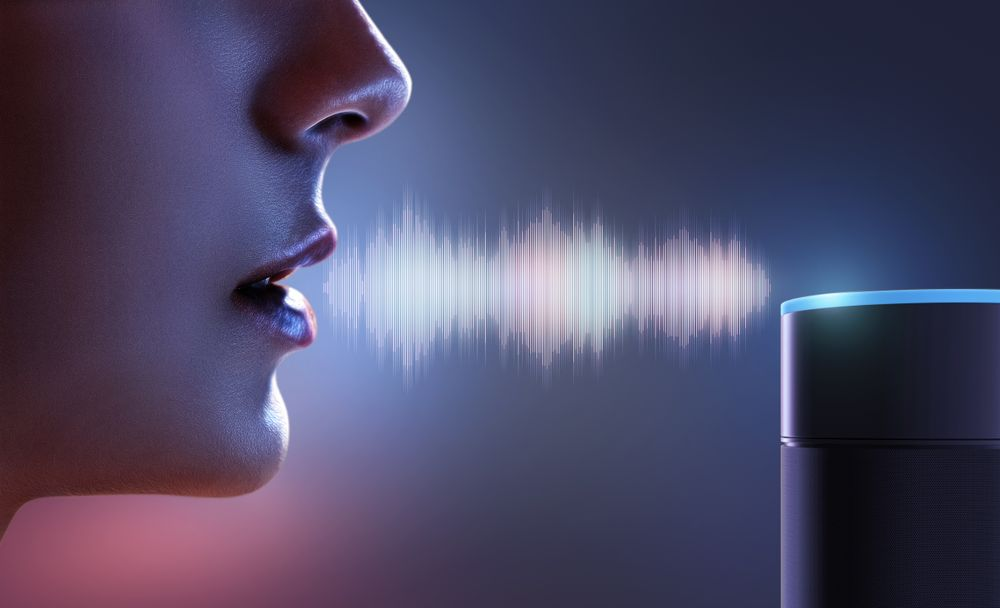
\includegraphics[width=0.75\textwidth]{images/VUI.jpg}
        \caption{Voice assistant using a VUI}
        \label{fig:VUI}
\end{figure}

A common method of gathering data about peoples views of a Voice Assistant is by analysing online product reviews. Experimental methods of this nature alone may not give a clear picture of the population as only certain groups of users may feel the need to leave a review, skewing the results. This research method was used to investigate users satisfaction and personification of the Amazon Echo \citep{purington_alexa_2017}. The authors of this work found some surprising results. They found that when technical errors were experienced, users were reluctant to continue using the device. It was assumed that these errors made people take notice of the device and its shortcomings, which caused people to not want to have to go to the bother of using it again. This dissertation will explore similar issues through its focus on perceived effort and the perception of `failing' to use a technology successfully. If technical issues require additional effort to overcome, then people may be put off from further use, because of frustration in overcoming the gulf of execution and the potential perception that they are `unable' to interact successfully.

A lab study undertaken by \citet{myers_patterns_2018} investigated the causes and impacts of the frustration caused by VUIs. The experiment involved participants interacting with the device in a laboratory setting and required them to undertake set tasks on three occasions. Common errors made by participants were recorded. Users didn't take notice of times when the device accepted their attempts to interact, indicating it achieved invisibility and had the potential to be acceptable. However, when users had to put extra effort in, they became annoyed; when it reoccurred in later occasions, their frustration was reinforced. The acceptability of this reduced usefulness was not examined and could be explored in this research, as being frustrated is rarely seen as acceptable in other aspects of life. The Lab setting and set tasks limited these results as conclusions may not be strongly valid for how users would use the interaction techniques in the wild.

\citep{myers_impact_2019}built on their previous work by exploring the limitations of the invisible nature of VUIs. Online responses and reviews were examined and an in-the-wild experiment was carried out to provide more ecologically valid results, in comparison to their previous lab study. This dual method will be attempted in my study of interaction methods, as both together can be ecologically valid by being in the wild while also gaining responses from large numbers of participants which may not have been possible to achieve due to the nature of using an interaction technique for an extended time.

From this initial investigation of voice assistants, it is clear that most studies focus on how people use them, with frustration and acceptability being emergent factors in the analysis. The reasons people may avoid using them have either not been explored, or been found by accident during analysis. This study will focus on the social reasons users may avoid using different novel interaction techniques through a combination of different experimental methods used by the above literature.

\subsection{Gestures}

Gestures are a non-verbal communication form, using meaningful body movements, posture, etc, to convey information, graphical examples are detailed in Figure \ref{fig:Gesture}. Gesture user interfaces similarly make use of body movements and postures for communication, in this case, to communicate intention to a computing device. Gestures can be sensed in several ways, impacting their form. The most common form is touch screen gestures, e.g., using multiple fingers, using varying pressures or tracing certain shapes. These are widely used by many devices and applications, and are generally socially acceptable. Device motion gestures (e.g., shaking or tilting a device for input) and mid-air gestures (e.g., waving a hand over a device or giving a thumbs-up) are two novel alternatives. These are less commonly used, although technology for sensing them is now commonplace in mobile devices. Motion and mid-air gestures are typically less socially acceptable than touchscreen interactions, likely in part due to being less common and requiring less subtle actions that might attract attention \citep{rico_usable_2010}.

\begin{figure}[!htb]
    \centering
    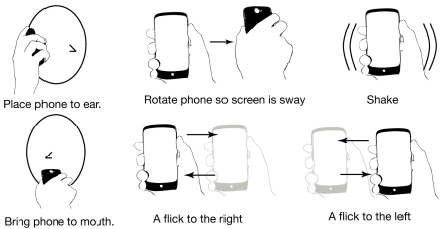
\includegraphics[width=0.75\textwidth]{images/gestures.png}
        \caption{Potential actions for gesture input}
        \label{fig:Gesture}
\end{figure}

The majority of previous literature has focused on gestures as not being socially acceptable in particular locations or in the presence of certain `audience' \citep{rico_usable_2010}. The social acceptability of an interaction is generally assessed by asking a participant to carry out various tasks in different scenarios, or by asking them to imagine themselves performing an interaction in those scenarios. The participants views are either recorded throughout the tasks \citep{ahlstrom_are_2014} or collected at the end using an interview \citep{rico_usable_2010}. Users can also be examined on various metrics to understand how well they carry out the gesture \citep{freeman_rhythmic_2017}. \citet{freeman_rhythmic_2017} detailed that mid-air gestures were very usable and completed easily when users were given instruction and found audio signals aligned well with their use due to the consistent eyes free nature of the features. This provides ground for the opportunity that users will be able to get more used to and more easily gain the benefits of Mid-Air Gestures. This will be explored with respect the the perceived social acceptance that is brought along with it.

Where gestures are performed is the focus of the study done by \citet{rico_usable_2010}. The author describes various types of gesture and explains why some of them are reasonable or should not be used. It is suggested that optimal gestures should mimic gestures that people may come across in their everyday life as they can be more familiar. Gestures that are found not to be effective are of an emblematic style as these may have preexisting meanings and could therefore be confused for their established connotations. Analysis will be done to maintain and solidify that using familiar gestures will make it easier for users to get used to using them, increasing their usefulness and therefore social acceptability.

Acceptance of an interaction method has also been found to have a strong correlation to where, with respect to their body, the user performs a gesture. \citet{ahlstrom_are_2014} found that if carrying out the gesture took more than 6~seconds, the user tends to not see it as acceptable, because it is more likely to attract attention. Gestures that require body movement more than a foot away from the body are also considered less acceptable. \citet{ahlstrom_are_2014} believe this to be purely for visual reasons as it may look unnatural to others and is more likely to attract unwanted attention. However, this could also indicate that users perceive an interaction technique to be socially unacceptable if they believe others around them will perceive them to be putting in an abnormal amount of effort to accomplish an interaction task. This will be explored through this dissertation research.

\subsection{Smart Glasses}

A wearable device is a broad term that covers devices such as Smart Glasses, Watches and Rings. Since these devices take the place of common fashion accessories they have an inherent need to be social acceptable. They must be  aesthetically pleasing, up to date with current trends and comfortable, all while facing the same interaction challenges of other devices, systems and applications. This study will focus only on the interactions with these types of devices, in particular Smart Glasses.

Research carried out by \citet{chuah_wearable_2016} attempts to understand the factors that determine the widespread adoption of smartwatches by the population. It was concluded that visibility and perceived usefulness are large factors in this adoption. This will be explored to establish if it is due to the user wanting to appear visible and not using effort by others which makes them confident in using the devices --- and similarly other novel interaction techniques --- in social situations. Other studies focused on smart glasses are in appearance that a device and its interaction modalities being unobtrusive enhance its social acceptance. This will be elaborated to understand if this is common for other interaction techniques and to decide if, over time, users will better understand interaction techniques to become more comfortable using them, even if they are slightly obtrusive, due to a new found familiarity.

The Focus of this area of study will be directed towards the social acceptability and the use fullness of the Snapchat Spectacles as the product was available to me, these are shown in Figure \ref{fig:Spectacles}. The product and its interaction methods have been vastly speculated in the technical community \citep{constine_why_2017}. It is often deemed that the product was a failure and never took off. It seems that even when people bought the device, they rarely used it consistently and often stopped using it after as little as a week \citep{constine_why_2017}. At this time there have been 3 iterations of the Spectacles and none of them have been close to being a common household item. The general consensus is that the fear brought about by other data glasses \citep{koelle_dont_2015}.

\begin{figure}[!htb]
    \centering
    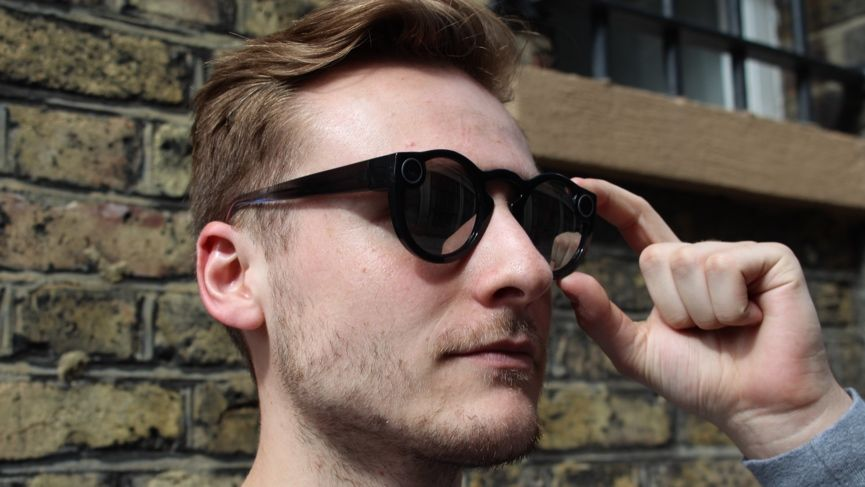
\includegraphics[width=0.75\textwidth]{images/spectacles.jpg}
        \caption{Snapchat Spectacles}
        \label{fig:Spectacles}
\end{figure}

\section{Effort, Usefulness and Acceptability}

There is a relationship between perceived usefulness and required effort; when solving a immediate problem, a person will view it in comparison to their background of probable future problems \citep{zipf_human_2016}.  If a person sees an outcome as having less worth than the effort required to conduct the required task, it is likely they will not see it as a useful thing to do and will not want to do it. \citet{zipf_human_2016} also suggests that it is the social norm that a person will strive to expend the least amount of energy to solve a problem and accomplish a goal.

If we view interaction through this lens, if the input action to a device requires more energy than what the desired output is worth, a user will not want to do it. Other literature strongly backs up this case in the context of personal user acceptance \citep{davis_perceived_1989}. \citet{zipf_human_2016} also believes that, ``A person is socially treated according to the social signals he emits''. This together with social norms of least effort, infers that one may not only want to reduce effort to conserve energy, but also so it does not appear to others that they are wasting it. This may mean they would get treated differently. It will be determined if reduction of energy consumption is purely for personal gain or if social pressures also have a part to play. 

 A study of attitudes among students gives similar insight into the relationship between perceived effort, usefulness and acceptance \citep{warrington_student_2000}. If one wants to be accepted by society, they must give off the correct norm of socially signals accordingly. In this study it is found that from a young age, we learn that the social norm is to put in the least viable amount of effort to accomplish a task. This dissertation will explore if the acceptance of technology is governed by similar `rules'. Social signals coming from the effort expelled when providing input through novel interaction techniques will be explored to understand if this is common among these circumstances. It may be socially desirable to minimise the amount of effort expended to accomplish an interaction task, to avoid being seen to be trying too hard.

These implications will be investigated in the context of novel interaction techniques, with particular focus on how their perceived usefulness and social implications vary over time. It is hypothesised that the more a person uses a new interaction method, they will become more used to using it and feel as though the desired outcome requires less effort and becomes more useful to them for accomplishing a task. Additionally, they may come across more more useful functions as time passes that were not evident before use, increasing the value they will get by using it (potentially meaning it is acceptable to use more effort). These together will imply that a user will perceive the task to become more useful over time and and less effort in comparison will be expelled, making it more socially acceptable to do. Acceptance growing over time is examined in detail by  \citet{hosokawa_walkman_1984}. This study details how over time, as people use or do something, it will gradually become more normal to them, it is referred to as ''The Walkman Effect''. Initial attitudes towards the Walkman were largely negative as it was a very out of the ordinary thing to use or be seen using in public. However, over time people became more familiar with it, as its clear function, usefulness, and ease of use leading to people being much more accepting of it. Before long, devices like this became the norm. This effect will be investigated to understand if the same may also be true for novel interaction techniques, which have yet to achieve widespread adoption.

\section{Summary}

Various attributes have been linked to social acceptability of Novel interaction techniques though an array of studies. Common attributes consist of interaction being carried out in specific circumstances that are deemed unacceptable and how noticeable the integration is to others around the user. There have been little to no links to Effort required or usefulness. Social norms of least effort have been widely documented for general social situations. These social norms of least effort will be further explored. A preliminary study will initially be carried out to gain an insight to people current perceptions of these links of effort ans social acceptability and which novel interaction technique it may apply to most adequately.

%==================================================================================================================================
\chapter{Preliminary Survey Study}

\section{Introduction}

A preliminary survey was conducted to investigate perceptions of novel interaction methods. The aims of this survey were to begin studying perceptions of perceived effort and social acceptability, and to inform the design of a later experiment. At this early stage of the project, there were three ideas for the main experiment:

\begin{description}
    \item[Smart-glasses] The potential for an evaluation of the participants usage and views of the Snapchat Spectacle wearable was considered, as this would not involve a substantial amount of technical development so could be done easily in conjunction with another method. This evaluation could collect data from different participants, detailing their frequency of use, opinion of usefulness and acceptability levels over some time. 

    \item[Speech] The opportunities of developing an application for either the Amazon Echo or Google Nest were investigated as both devices were available to me and have been widely adopted in recent years. A potential study would explore how participants use the device. For example, did they attempt to use speech all the time, or did they simply control the speaker within the assistant and other devices using their mobile device as a remote. 

    \item[Gestures] Another possible option for the experiment was to develop an app that would make use of some type of gesture interface. This could be Touch Gestures, Mid-Air Gestures or Device Motion Gestures. The experiment could cover usage and opinions of the features and interaction style, also looking into ease of use, usefulness, and social acceptability.
\end{description}

The survey therefore aimed to explore perceptions surrounding these interaction methods, to inform the main evaluation in this project. It would also gather data about familiarity, prior experience, and preference for using these interaction modalities, as this would likely have an impact on perceptions of usefulness and acceptability.

\section{Methodology}

A survey was created and distributed to a sample of 24 participants, varying in age, gender, and technical knowledge. Participants were briefed on the aims of the research as a whole, as well as the aims of the specific questionnaire. Consent was granted by all participants and they were informed that they may withdraw from the process at any time, they were directed to the relevant people had they had any questions throughout, as per the ethics checklist. 

At the start, participants were asked to detail their views on how the effort a task takes affects their likelihood to complete it (in general, rather than specifically related to interaction). They were asked to elaborate on if they had ever avoided putting effort into a task for social reasons and if they were aware of a social slur surrounding this issue of avoiding applying excess effort to a task.

Following this, users were asked to gauge on a Likert scale how socially acceptable using certain novel interactions in a specific location may be. This was then also asked for the case of the same task outcome and situation but simply using the touch screen alternative method on their mobile device, as opposed to the novel interaction technique. They were asked about the relative effort compared in the two circumstances. They were asked to detail if they frequently use any of the range of interaction techniques and given the opportunity, in what circumstances they would happily use them and perceive it to be socially acceptable.

Finally, participants were asked to recommend what Gestures they would see fit for various functions that do not currently have associated with gestures in common devices. These were targeted to the functions that could be used in an app that could be created with integrated gesture input potential.

\section{Results}
Participant responses to the survey questions were transferred to an Excel Spreadsheet, removing erroneous or incomplete data in the process. Analysis of responses is presented in the following sections, structured by theme.

\subsection{Social norms related to perceived effort}

Half of the participants would not see it as appealing to undertake a task which required more effort than the output. An additional third thought that others, be it colleagues or fellow students or sports team members etc, would look at them badly for putting in this effort, detailed in Figure \ref{fig:reward}. This reinforces the idea that people believe there to be a social norm that you should avoid putting in extra effort when you do not need to. 

\begin{figure}[!htb]
    \centering
    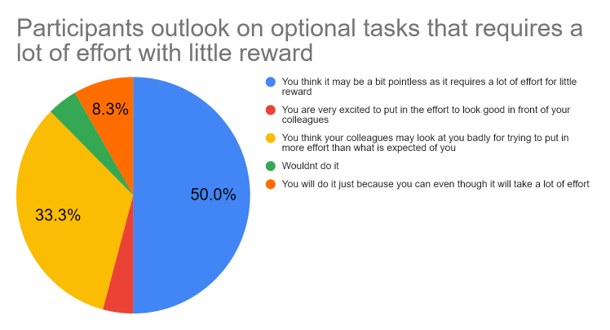
\includegraphics[width=\textwidth]{images/littleReward.png}
    %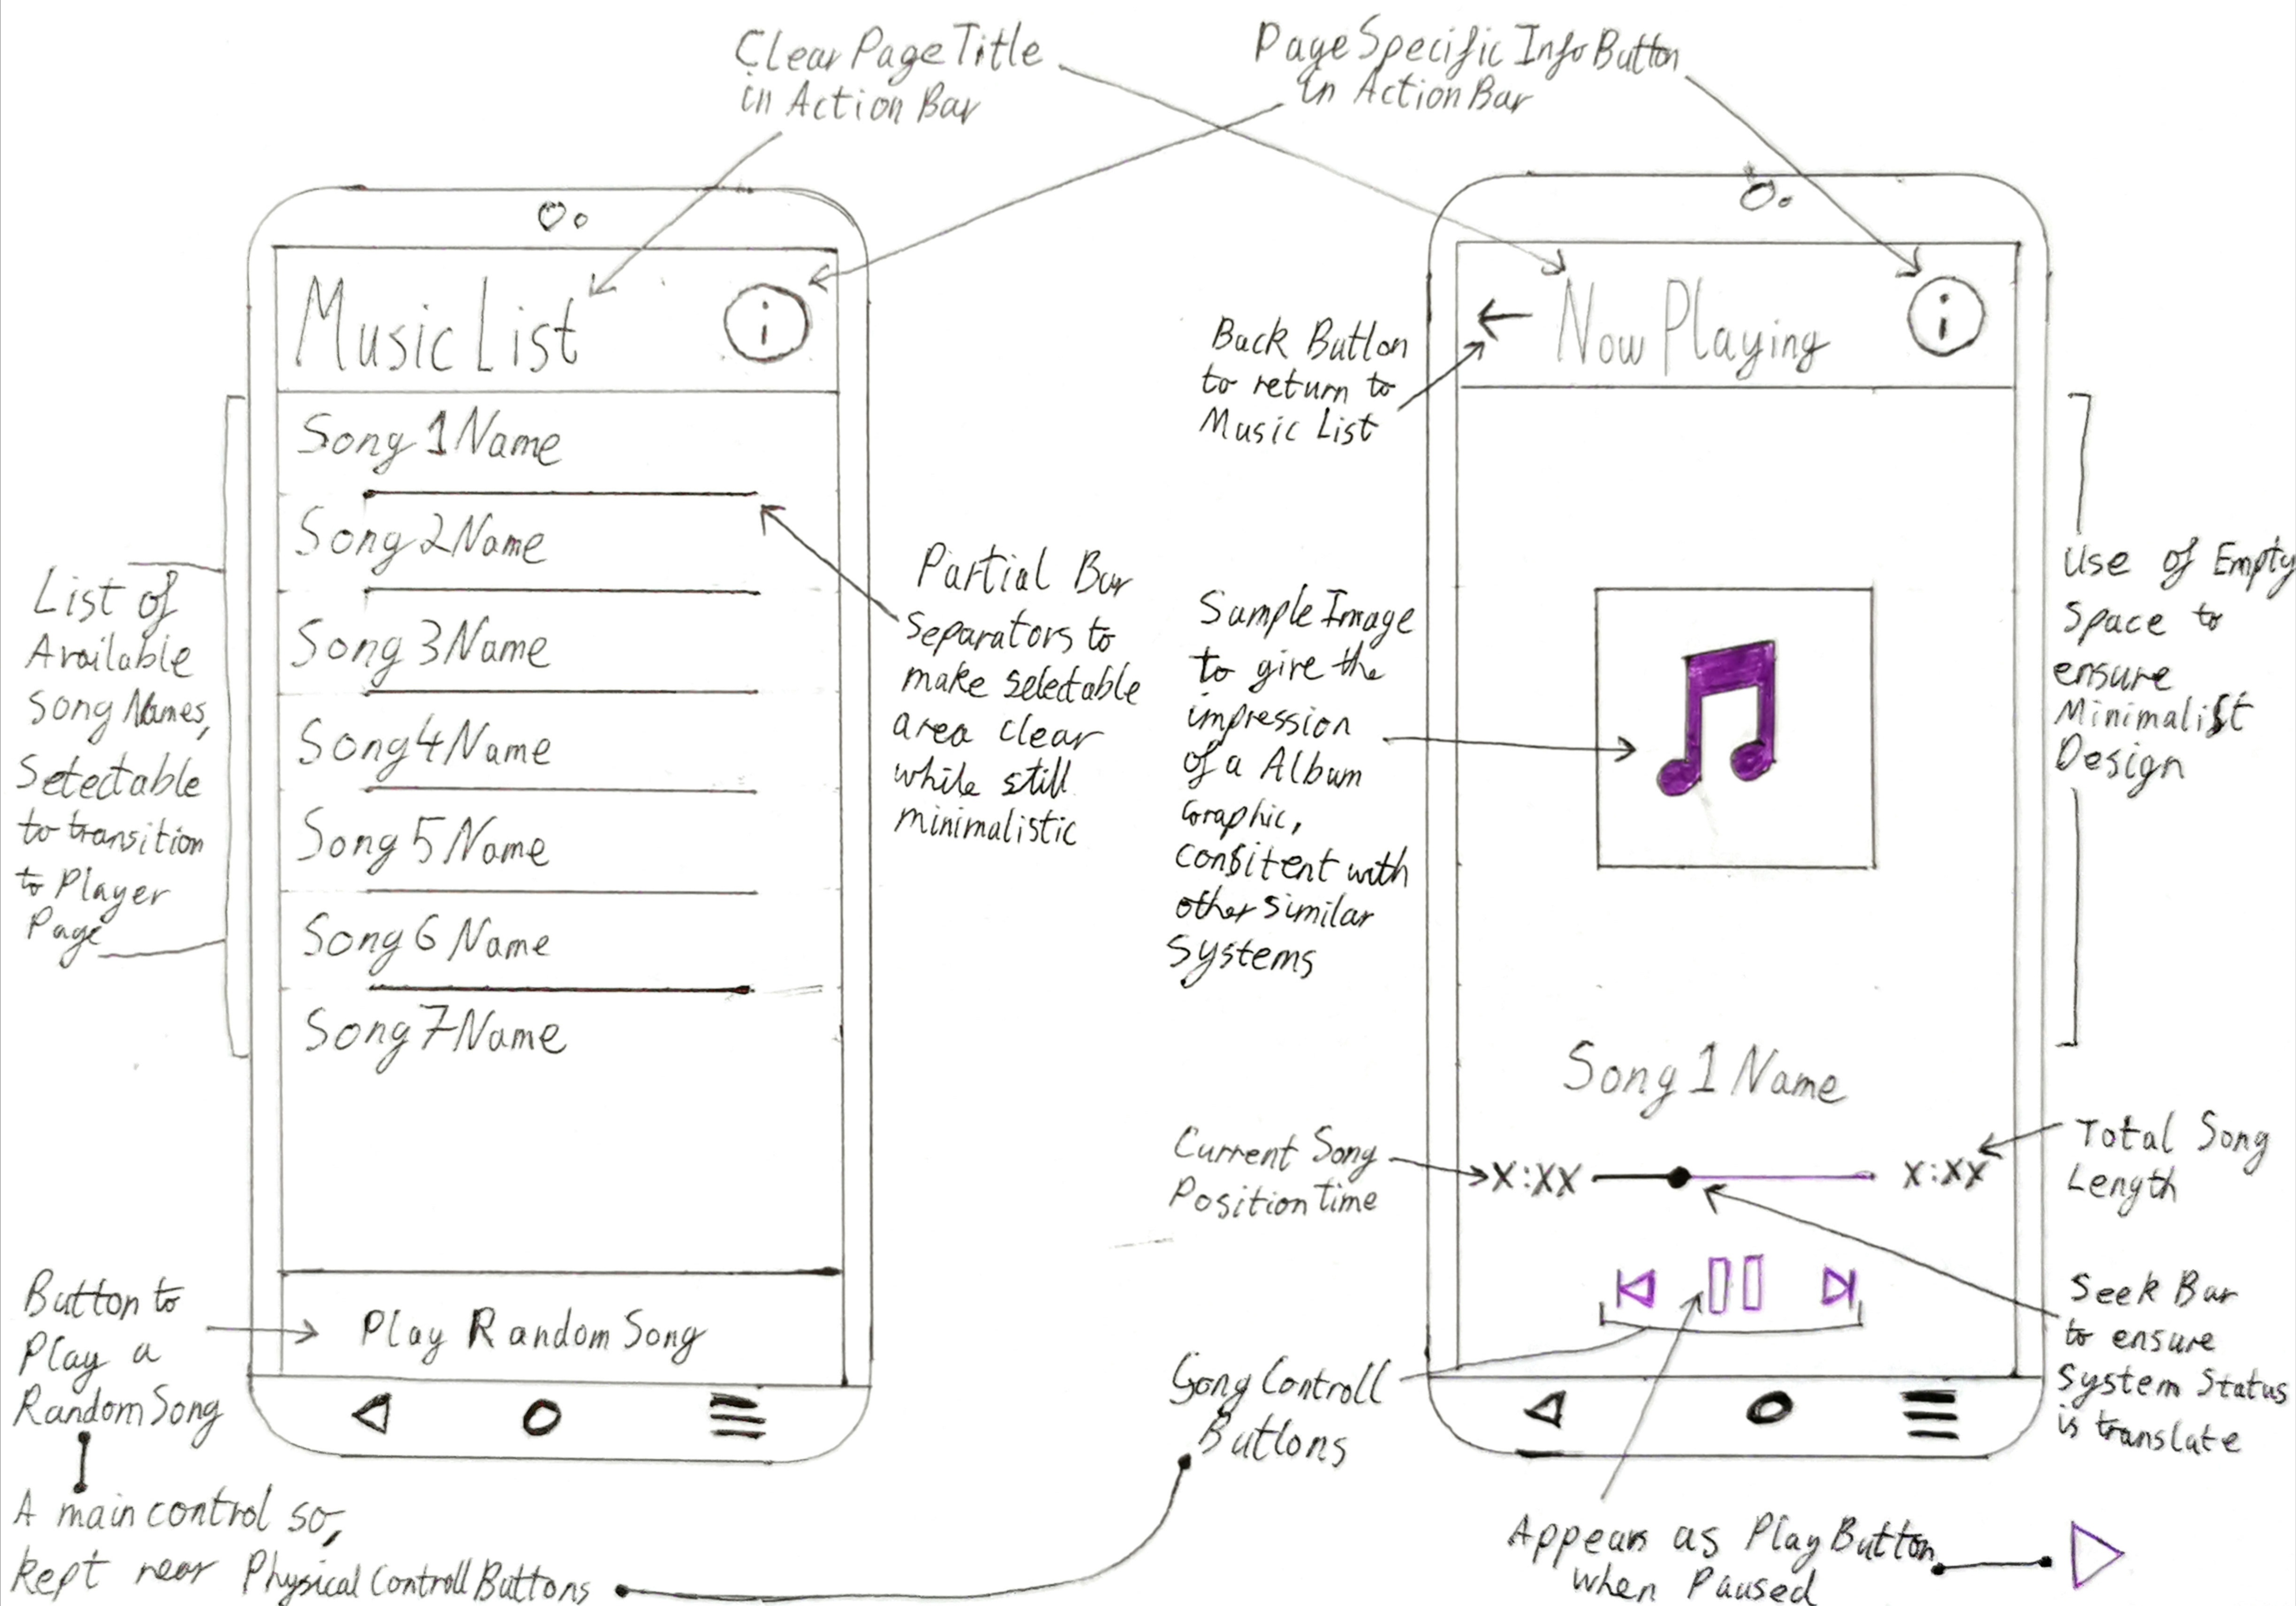
\includegraphics[width=\textwidth]{images/papWF.jpg}
        \caption{Details of participants responses to the question "You are given an optional task that requires a lot of effort (eg. an optional exercise at college/University or an optional unpaid training session at work). Select from the following which best describes how you would feel about it?". Optional responses are detailed in the legend.}
        \label{fig:reward}
\end{figure}

Only two of the participants said that they had never avoided appearing as though they had put in more effort into a task than what was required. Many of the participants gave examples of when they do this, some included hiding how much you study for tests, how hard you they tried to get a job and even so not to appear like they need to put in extra work in case others think they are struggling. Building on the idea that people do not want to appear as though they are trying harder than necessary to complete a task. The results also introduce the idea that people do not want to look like they must practice too much and put in too much effort to get good at something. People want to make it look like what they are doing has been done easily. 

The participants were presented with a name someone may call another if they feel as though they are going over and above what is expected them. Every single participant knew its connotations and were able to explain that they were negative. People are very aware of the norms of "trying too hard" to do something and the repercussions of doing so. Many people are sucked into this way of thinking and it has become accepted that one must not appear to be trying too hard to achieve something, be it their life goals or a small daily task.

\subsection{Perceptions of acceptability of novel interaction methods}.

There seemed to be some confusion understanding questions related to technologies participants were aware of and technologies participants use on a weekly basis. Some participants did not say that they were aware of some technologies, yet said that they used them on a weekly basis. Following the surveys closure to additional responses, participants were asked some additional questions about the survey, this included them detailing their understanding of this question. It was noted that some participants thought that Question 13 meant they were to select what technologies they were only aware of and had never used. It can therefore inherently be assumed that where a participant uses a technology on a weekly basis that they also are aware of it. With these adjustments, all participants stated they were aware of Voice assistants with 70.8\% using them on a weekly basis. Half of the participants were aware of Gestures with only a quarter claiming to use gestures on a weekly basis. All but 2 participants were aware of what Virtual reality was yet only 2 claiming to use it on a weekly basis. A total of 54.2\% of users were aware of the Snapchat Spectacles, with again only 2 claiming to use them on a weekly basis. No participant was unaware of any of these technologies but 6 participants did say that they did not use any of them weekly.

For questions relating to how users perceive using a shuffle feature on a mobile device, a total of 91.67\% of people rated using a mobile phones touch screen interface a five out of five for acceptability with the remaining , participants rating it a four. Suggesting people are very familiar with using a touch screen interface and see no reason to why it would be unacceptable to use. The average acceptability rating of using a device motion gesture was 4.25, slightly less than than the touch screen alternative rating of 4.92. This is not a substantial difference yet does still infer that there is less confidence around using gestures. When determining what users believe to use more effort there was a 45.8\% to 54.2\% split. This may infer that users have a very varying opinion of the use of touch screen versus motion gesture. This could be down to users unfamiliarity of the technology as 75\% of participants claimed that they do not use them on a weekly basis. It was stated that the most common reasons for a person not to use a gesture was if they were unhelpful (70.8\%) or not easy to use (66.7\%). Less than 17\% believed that company would effect this and only an eighth of users thought their location would change their mind not to use gestures. This was considerably less than the other interaction methods.

When asked about their perceptions of taking pictures and short videos when on a walk with friends, the average rating of how acceptable it is to take a picture with your phone was 4.58 on a five point scale, determining users find this very acceptable. On the other hand, participants gave wearing and using the wearable, Snapchat Spectacles, an average rating of less than 2. Inferring many people believe this to be a particularly unacceptable. Over 70\% of participants were under the impression that wearing the Spectacles would be more effort that simply taking your phone out and taking a picture with that. This could very well be the reason for people finding this method unacceptable. Users reasons to decide not to use spectacles backs this up. A total of 75\% of participants felt that the technology not being useful and taking a lot of effort with respect to the desired outcome would change their mind about using the technology. Again falling in line with two thirds of participants believing it not being easy to use to be a strong reason to avoid using the technology. Less than 30\% said that using the spectacles in unfamiliar company would make them rethink its use and only a quarter feeling that they would be affected by the location. 

Questioning participants about setting a timer produced the following responses. Setting an alarm on a mobile phone using the devices touch screen received a high average acceptability rating of 4.79 of of 5 from the participants. Doing the same task using a voice assistant received a moderate average rating of 3.54 of of 5. There was a further agreement with users in that using the voice assistant takes more effort, with only just over a third believing it is easier to use the voice assistant. This correlates well with the individual ratings as they seem to be very segregated. A third of participants rated the voice assistant a 5 for acceptability, a single parson rated it 2 and the remainder rated it a 3 out of 5. In general, where participants rated Voice assistants 2 or 3 they said it would take more effort to use than the phone and conversely for participants giving it a rating of 5. This had vary little variation suggesting there is a very divided view of Voice assistants. It was thought that this might be due to users familiarity of using VAs by either learning that they were not as easy to use as they appeared and used a lot of effort or by learning that they took little effort to use. Yet it was found that there did not seem to be a great correlation between these two attributes where the users were familiar. However, there was only one person that was not familiar with the technology and thought it would take less effort. While the other 6 that were unfamiliar with VAs thought it would take more effort than the mobile phone's touch screen alternative. Participants perception of VAs use being avoided due to it not being useful or not easy to use --- just over half for both). However the company the user is in did seem to affect the participant's opinions more than in other technologies.

\subsection{User Gesture preferences and suggestions}

There seemed to be some confusion understanding questions related to technologies participants were aware of and technologies participants use on a weekly basis. Some participants did not say that they were aware of some technologies yet said that they used them on a weekly basis. Following the surveys closure to additional responses, participants were asked some additional questions about the survey, this included them detailing their understanding of this question. It was noted that some participants thought that Question 13 meant they were to select what technologies they were only aware of and had never used. It can therefore inherently be assumed that where a participant uses a technology on a weekly basis that they also are aware of it. With these adjustments, all participants stated they were aware of Voice assistants with 70.8\% using them on a weekly basis. Half of the participants were aware of Gestures with only a quarter claiming to use gestures on a weekly basis. All but 2 participants were aware of what Virtual reality was yet only 2 claiming to use it on a weekly basis. A total of 54.2\% of users were aware of the Snapchat Spectacles, with again only 2 claiming to use them on a weekly basis. No participant was unaware of any of these technologies, but 6 participants did say that they did not use any of them weekly.

For questions relating to how users perceive using a shuffle feature on a mobile device, a total of 91.67\% of people rated using a mobile phones touch screen interface a five out of five for acceptability with the remaining, participants rating it a four. Suggesting people are very familiar with using a touch screen interface and see no reason to why it would be unacceptable to use. The average acceptability rating of using a device motion gesture was 4.25, slightly less than the touch screen alternative rating of 4.92. This is not a substantial difference yet does still infer that there is less confidence around using gestures. When determining what users believe to use more effort there was a 45.8\% to 54.2\% split. This may infer that users have a very varying opinion of the use of touch screen versus motion gesture. This could be down to user’s unfamiliarity of the technology as 75\% of participants claimed that they do not use them on a weekly basis. It was stated that the most common reasons for a person not to use a gesture was if they were unhelpful (70.8\%) or not easy to use (66.7\%). Less than 17\% believed that company would affect this and only an eighth of users thought their location would change their mind not to use gestures. This was considerably less than the other interaction methods.

When asked about their perceptions of taking pictures and short videos when on a walk with friends, the average rating of how acceptable it is to take a picture with your phone was 4.58 on a five-point scale, determining users find this very acceptable. On the other hand, participants gave wearing and using the wearable, Snapchat Spectacles, an average rating of less than 2. Inferring many people believe this to be a particularly unacceptable. Over 70\% of participants were under the impression that wearing the Spectacles would be more effort that simply taking your phone out and taking a picture with that. This could very well be the reason for people finding this method unacceptable. Users reasons to decide not to use spectacles backs this up. A total of 75\% of participants felt that the technology not being useful and taking a lot of effort with respect to the desired outcome would change their mind about using the technology. Again, falling in line with two thirds of participants believing it not being easy to use to be a strong reason to avoid using the technology. Less than 30\% said that using the spectacles in unfamiliar company would make them rethink its use and only a quarter feeling that they would be affected by the location. 

Questioning participants about setting a timer produced the following responses. Setting an alarm on a mobile phone using the devices touch screen received a high average acceptability rating of 4.79 of 5 from the participants. Doing the same task using a voice assistant received a moderate average rating of 3.54 of 5. There was a further agreement with users in that using the voice assistant takes more effort, with only just over a third believing it is easier to use the voice assistant. This correlates well with the individual ratings as they seem to be very segregated. A third of participants rated the voice assistant a 5 for acceptability, a single parson rated it 2 and the remainder rated it a 3 out of 5. In general, where participants rated Voice assistants 2 or 3 they said it would take more effort to use than the phone and conversely for participants giving it a rating of 5. This had very little variation suggesting there is a very divided view of Voice assistants. It was thought that this might be due to user’s familiarity of using VAs by either learning that they were not as easy to use as they appeared and used a lot of effort or by learning that they took little effort to use. Yet it was found that there did not seem to be a great correlation between these two attributes where the users were familiar. However, there was only one person that was not familiar with the technology and thought it would take less effort. While the other 6 that were unfamiliar with VAs thought it would take more effort than the mobile phone's touch screen alternative. Participants perception of VAs use being avoided due to it not being useful or not easy to use --- just over half for both). However, the company the user is in did seem to affect the participant's opinions more than in other technologies.

\subsection{User gesture preferences and suggestions}

Users were provided with mobile device functions that are ordinarily controlled though touch screen or other hardware interaction. They were asked to provide an example of a gesture alternative that they felt would naturally fit that function. Responses were coded into 5 categories; (1)~ No Answer, (2)~ Touch Gesture, (3)~ Mid-Air Gesture, (4)~ Device Motion Gesture, and (5)~ Other. It must also be noted, during error correction, if a gesture was out of the reasonable technical scope or did not include a gesture, the response was counted as no answer unless any additional opinion is stated.

Participants were given the hypothetical task of adjusting the volume. Instead of pressing the volume up button, 8 participants opted for a touch gesture, 6 for Mid-Air and 5 for device motion. 5 participants gave no response. Instead of pressing the volume down button, 7 participants opted for a touch gesture, 7 for Mid-Air and 5 for device motion. 5 participants gave no response, and one provided an alternative option. To adjust the volume people, tend to want to use the touch screen and Mid-air gestures over device motion gesture. This is likely to be due to the more controllable nature of these interaction types over definitive intervals. This would suit the nature of volume adjustments.

When presented with the opportunity to skip to the next song playing on the device, 6 participants were unable to provide and answer. 8 provided a touch-based solution, 5 provided a Mid-Air Gesture, 4 opted for a device motion gesture and a single participant responded with a solution that was considered Other. Most answers were reverting to various touch options, suggesting that the participants were failing to think of more innovative ideas of what gestures could represent this task. The number of answers for Mid-Air and Motion Gestures were both low with Mid-Air Gestures having a slight edge in preference.

Users were tasked with stating an alternative method of pausing and playing music. 7 participants supplied a response under the No Answer category and 2 under Other. 8 recommended a Touch gesture with only three favouring both Mid-Air and Device Motion style gestures. The number of participants that did not give an answer of a gesture increased. This suggests that the participants were running out of creative ideas to answer with, most answers reverting to various touch options, again reiterating that the participants losing interest. The number of answers were again low for Mid-Air and Motion Gestures.

Overall, there is a lack of results of device motion gestures. It is thought that the results are biased against this due to many people being unfamiliar with the use of gestures. In general device motion gestures are infrequently used within current technology so many of the participants may not be familiar with its potential and therefor failed to give an answer including it. Answers that did include device motion gestures tended to be more in detail which also suggests that it may be participants that are more familiar with the capabilities that suggested them.

\section{Discussion}

Participants seemed aware of the social norms of least effort. This supports the reasoning for exploring how these social norms may come into play when considering the social acceptability of novel interaction techniques.

It was decided that the focus of this research project will be Mid-Air and Device Motion Gestures. Many factors were considered when making this decision. Voice assistant interactions were found to already be commonly used among the participants with many already being familiar with their use and having already formed strong opinions about their utility and acceptance. Experimentation with Snapchat Spectacles would not be reliable. Only one device was available and to ensure a reliable sample size, users would not be able to use them for a sufficient time to become familiar with them to detect a substantial change in opinion and visa versa. There seemed to be no resolve for this trade off. This method would also lack external validity as claims could only be made about this specific device due to its individuality. Gestures of such type were found to be the most practical and safe option during the Covid-19 pandemic. Users will be able to download an Android app which will implement Mid-Air and Device Motion Gestures without the need for any physical meeting or exchange of a device. 

Users appeared to understand these types of interactions without having experience using them. This would enable the potential for participants to increase their current use if the interaction technique and therefore introduce the ease of use and usefulness that will be found. These attributes effects on social acceptability would be measured over time. This lack of prior knowledge of these gesture types was shown in participants responses in the survey, they were unable to consistently provide reasonable gestures that could be used. 

Inspiration for the gestures that will be implemented was taken from survey responses and guidelines from other appropriate literature \citep{rico_usable_2010}. Gestures will be made to be familiar to users through being similar motions to other tasks yet without being emblematic of hand signals that may already have social meanings in society. A shake style Device Motion Gesture will be developed to initiate playing a random song in a media player. This is inspired by the shaking motion one may make before rolling dice, the result of each being a random outcome. It will be possible to pause or play a song by holding a hand in front if the device, taking inspiration from both user responses and the stop sign one may use (e.g., a police officer stopping a vehicle). These share the common trait on directing something stop.

%==================================================================================================================================

\chapter{Technical Development}

\section{Overview}
Android was chosen as a development platform to enable the experiment to take place remotely using a user's own device. This application would enable users to interact using Mid-Air and Device-Motion Gestures. The app that was created was based on a music player application, because many people use these types of apps frequently and would be familiar with the standards functions available. Since the intended use of the app was for a longitudinal evaluation, the app needed to provide functionality that people were likely to use frequently. The following details the process in which the required application was developed. It notes the decisions made, particularly when issues were encountered, as well as the testing that was carried out and the reasoning for it. The application would be named Motion Music.

\section{Platform}

The focus of this development would be to create an smartphone app. Android was chosen as the development platform because of the widespread adoption of Android mobile devices, making it easier to recruit evaluation participants. The application would be developed using the Android Studio IDE. Android Studio supplies a unified environment to build, test and debug applications, as well as providing emulators to run the application on. This can improve the swiftness of creation as the application is not required to be downloaded onto a real-world device to understand what it looks like and how it will function. Some basic knowledge is known about its use, allowing me to build on my previous experience with smartphone app development.

Due to the nature of the application, music assets needed to be sourced. I chose to provide music files so that participants would have media files to use in the app, since these may not be available already due to use of streaming apps instead. The platform that was used for this was ccMixter operated by ArtisTech Media... . This is a site that provides free-licensed audio samples for commercial and non-commercial use. It provides creative proper means of attributions and crediting for the purpose of the Creative Commons License which covers all audio files available on the site. This platform was one of many of a similar style that could have provided the appropriate platform. This one was chosen as it had various documentation detailing how to use correctly and legally, what the creators and contributors provide.

For designing of the appearance of the application, wire frames and prototypes were required. To ensure they were completed to a standard to be able to evaluate them a digital platform was adopted for their creation. The Figma desktop app was used as there was a free student version available with no time restriction. Ultimately it was found to be a more advanced system with a much more realistic end product, leading to quality prototypes.

% EF: just a comment to remind me where I got to...

\section{Process}

The application was created with the User Study in mind and was named Motion Music. Initial design of what the appearance and workflow of the application was created through a process of creating low fidelity wire-frames followed by high fidelity digital wire-frame prototypes. Following this, various assets that would be used by the application were accumulated to ensure the implementation process was not hindered by hte assumption of how the music files would be supplied to the participants. The application was then implemented and ongoing and final testing and evaluation of both the initial music application and the additional gesture integration with it was carried out.

\subsection{Design}

Ensuring that usability of the base app was essential in this development. It was vital that no part of the app was unusable or caused problems for the user. If this was the case, then the data that would be collected would inevitably be skewed and false. Information collected and users’ opinions over time should solely be on directed towards the gestures that would be incorporated and not any other part of the system. For these reasons it was appropriate to create low fidelity paper wireframes and a digital prototype. The 10 usability heuristics were considered throughout.

Initially, simple low fidelity paper wire-frames were created. Examples of such are shown in Figure \ref{fig:paperWF}. These were useful to gain an understanding of what the app could look like and how users would want to use it. It helps to understand the flow of the applications. These types of wireframes are effective at the early stage of the development as they can be created in a very short time and use few resources. They can be adapted in very little time to adjust to various needs as problems are encountered or more efficient solutions are found. Initially there was a home page leading to options of 3 pages (1)~ Tunes, (2)~ Artists list and, (3)~ Information. The Tunes page would show a list of all songs available. The Artist page would show a list of all artists which would then lead to a further page showing all that specific artists songs. The information page would detail the purpose of the application and how to use it. When a song was clicked via the song or artist page, this would initiate the playing of that song and open the player page. On this page there would be options to pause, play, skip to the next song in the list and play the previous song in the list. There would also be a seek bar. The user would also be able to go back to the song or artist page they first clicked a song on to view other songs. This was ultimately changed to a single central tunes list page. This decision was made as it could not be guaranteed that all audio files on all users’ devices would have been assigned both a name and an artist to be categorised by. It also seemed much more streamlines as opposed to the hierarchical initial design. Each page would have its own designated information page, accessible on the action bar. The Random Song button was also added to the tunes list page.

\begin{figure}[!htb]
    \centering
    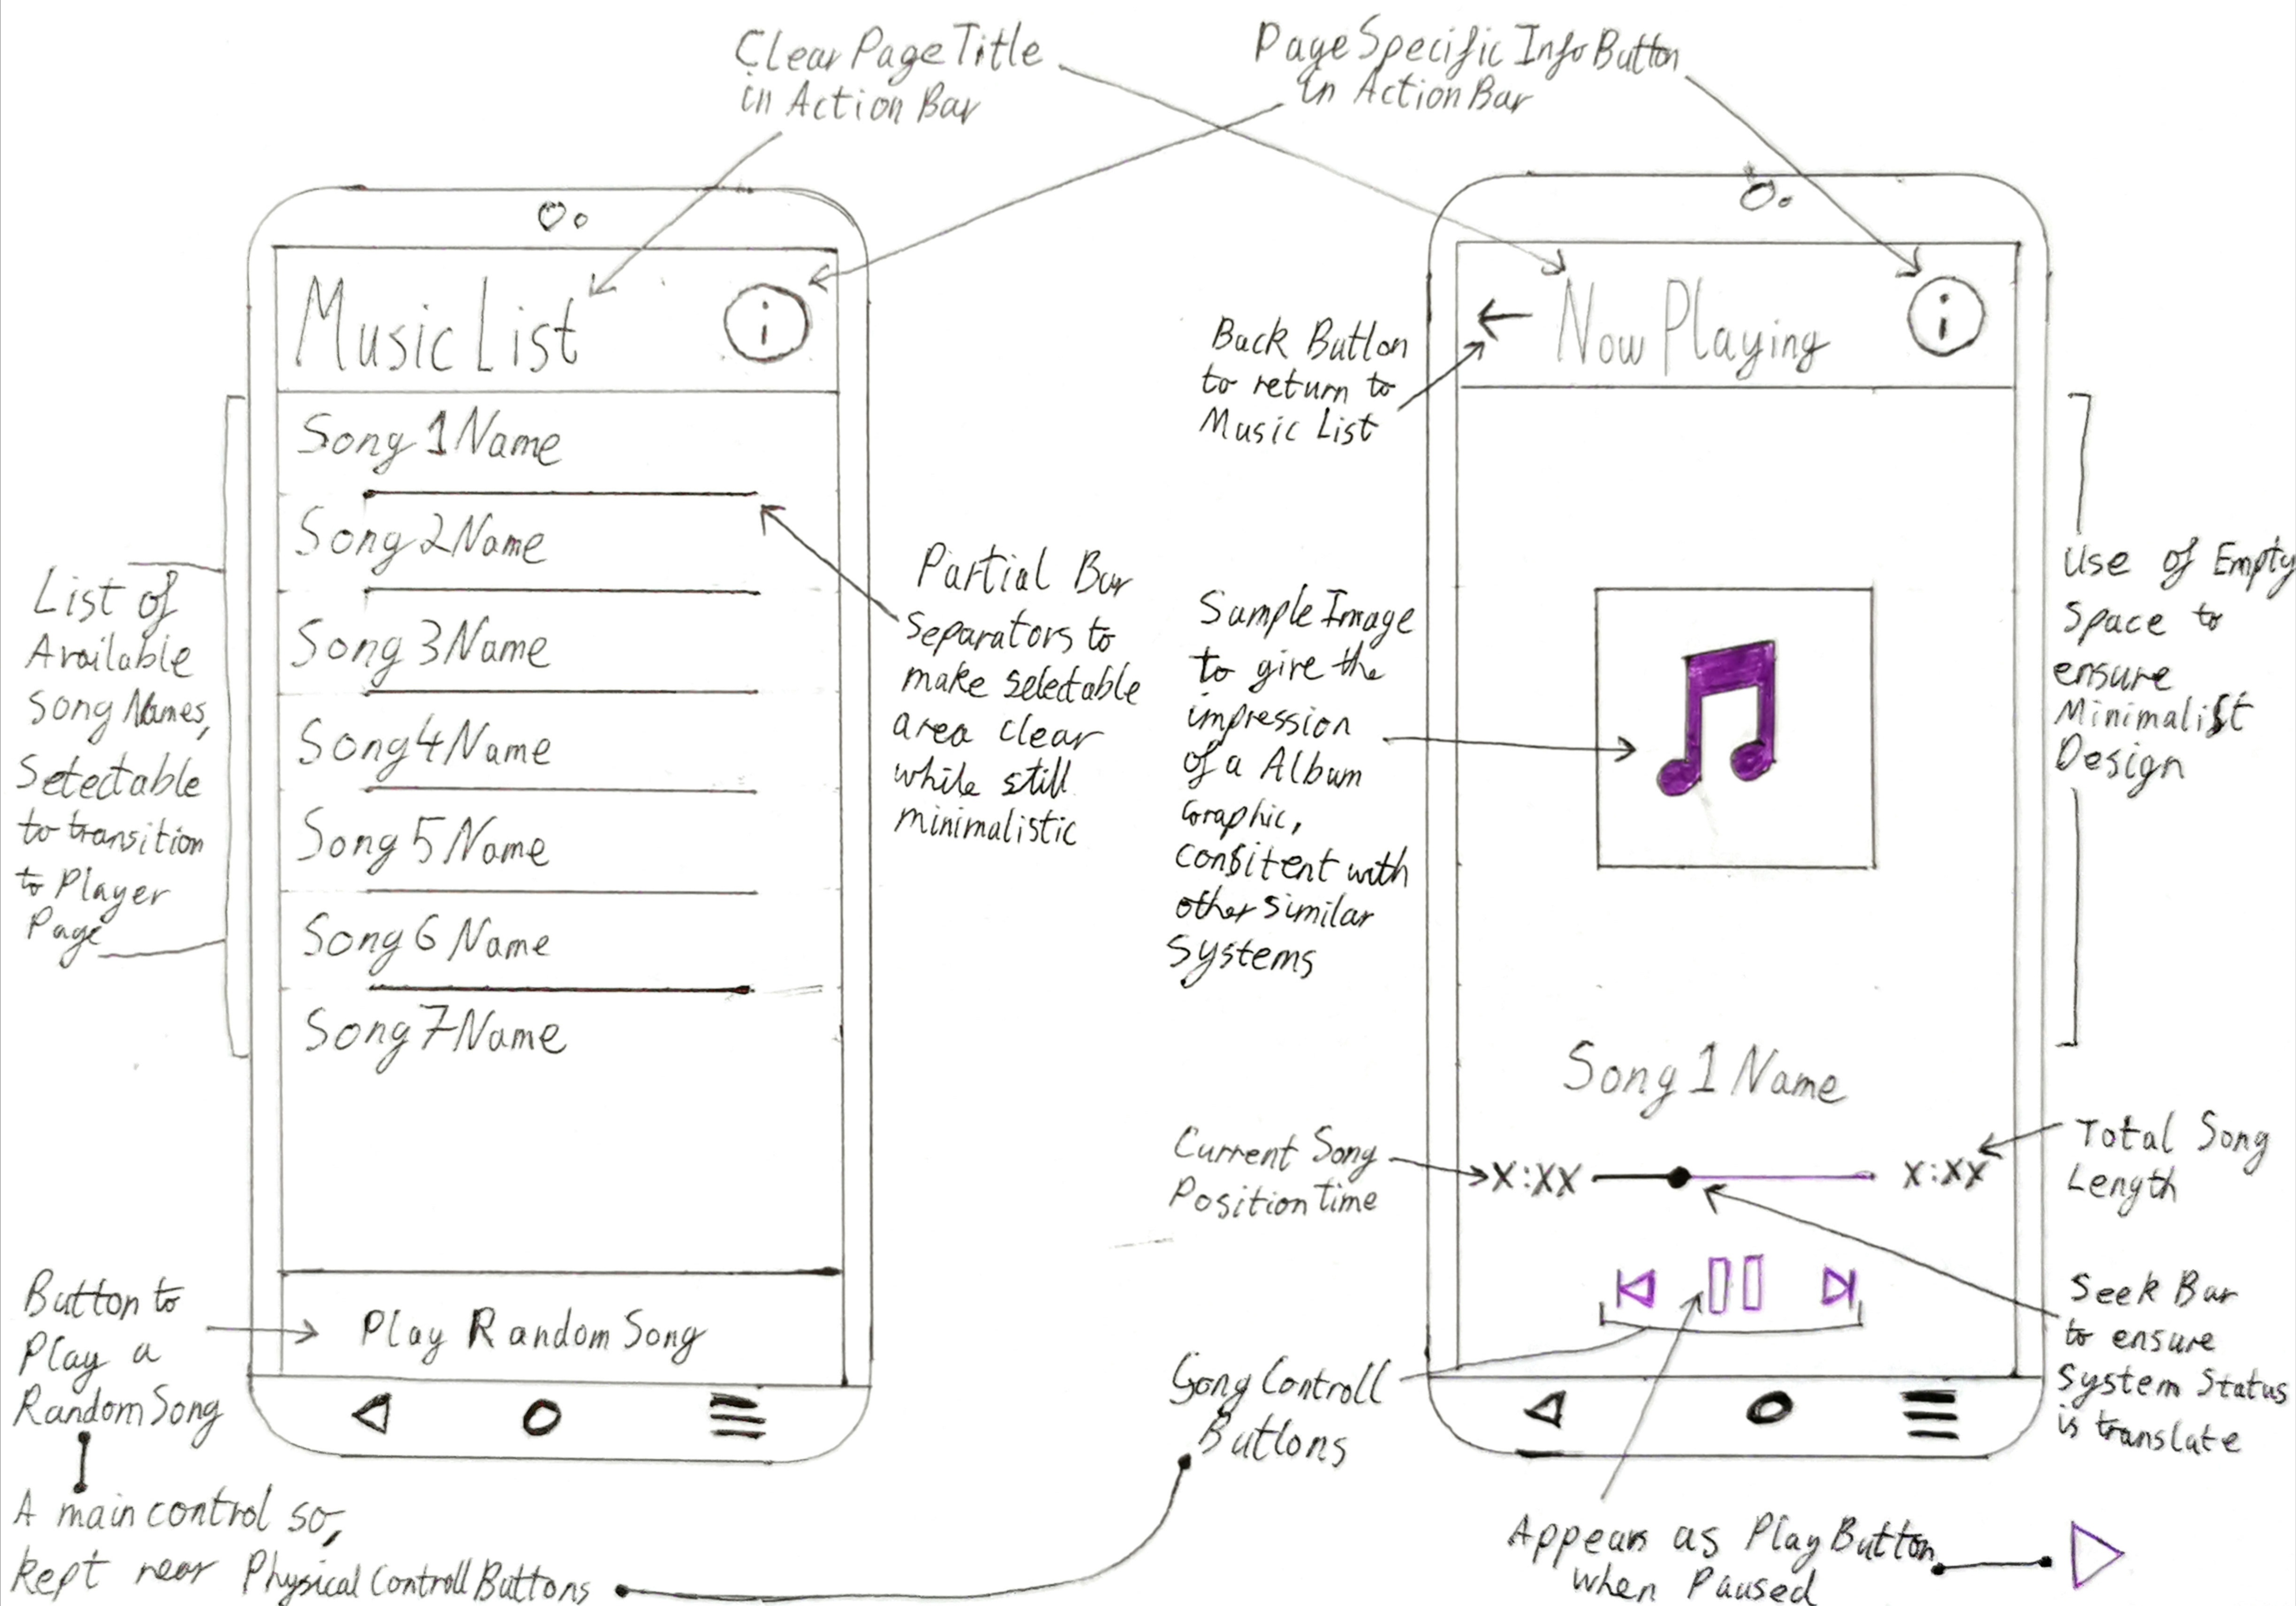
\includegraphics[scale=0.0675]{images/papWF.jpg}
    %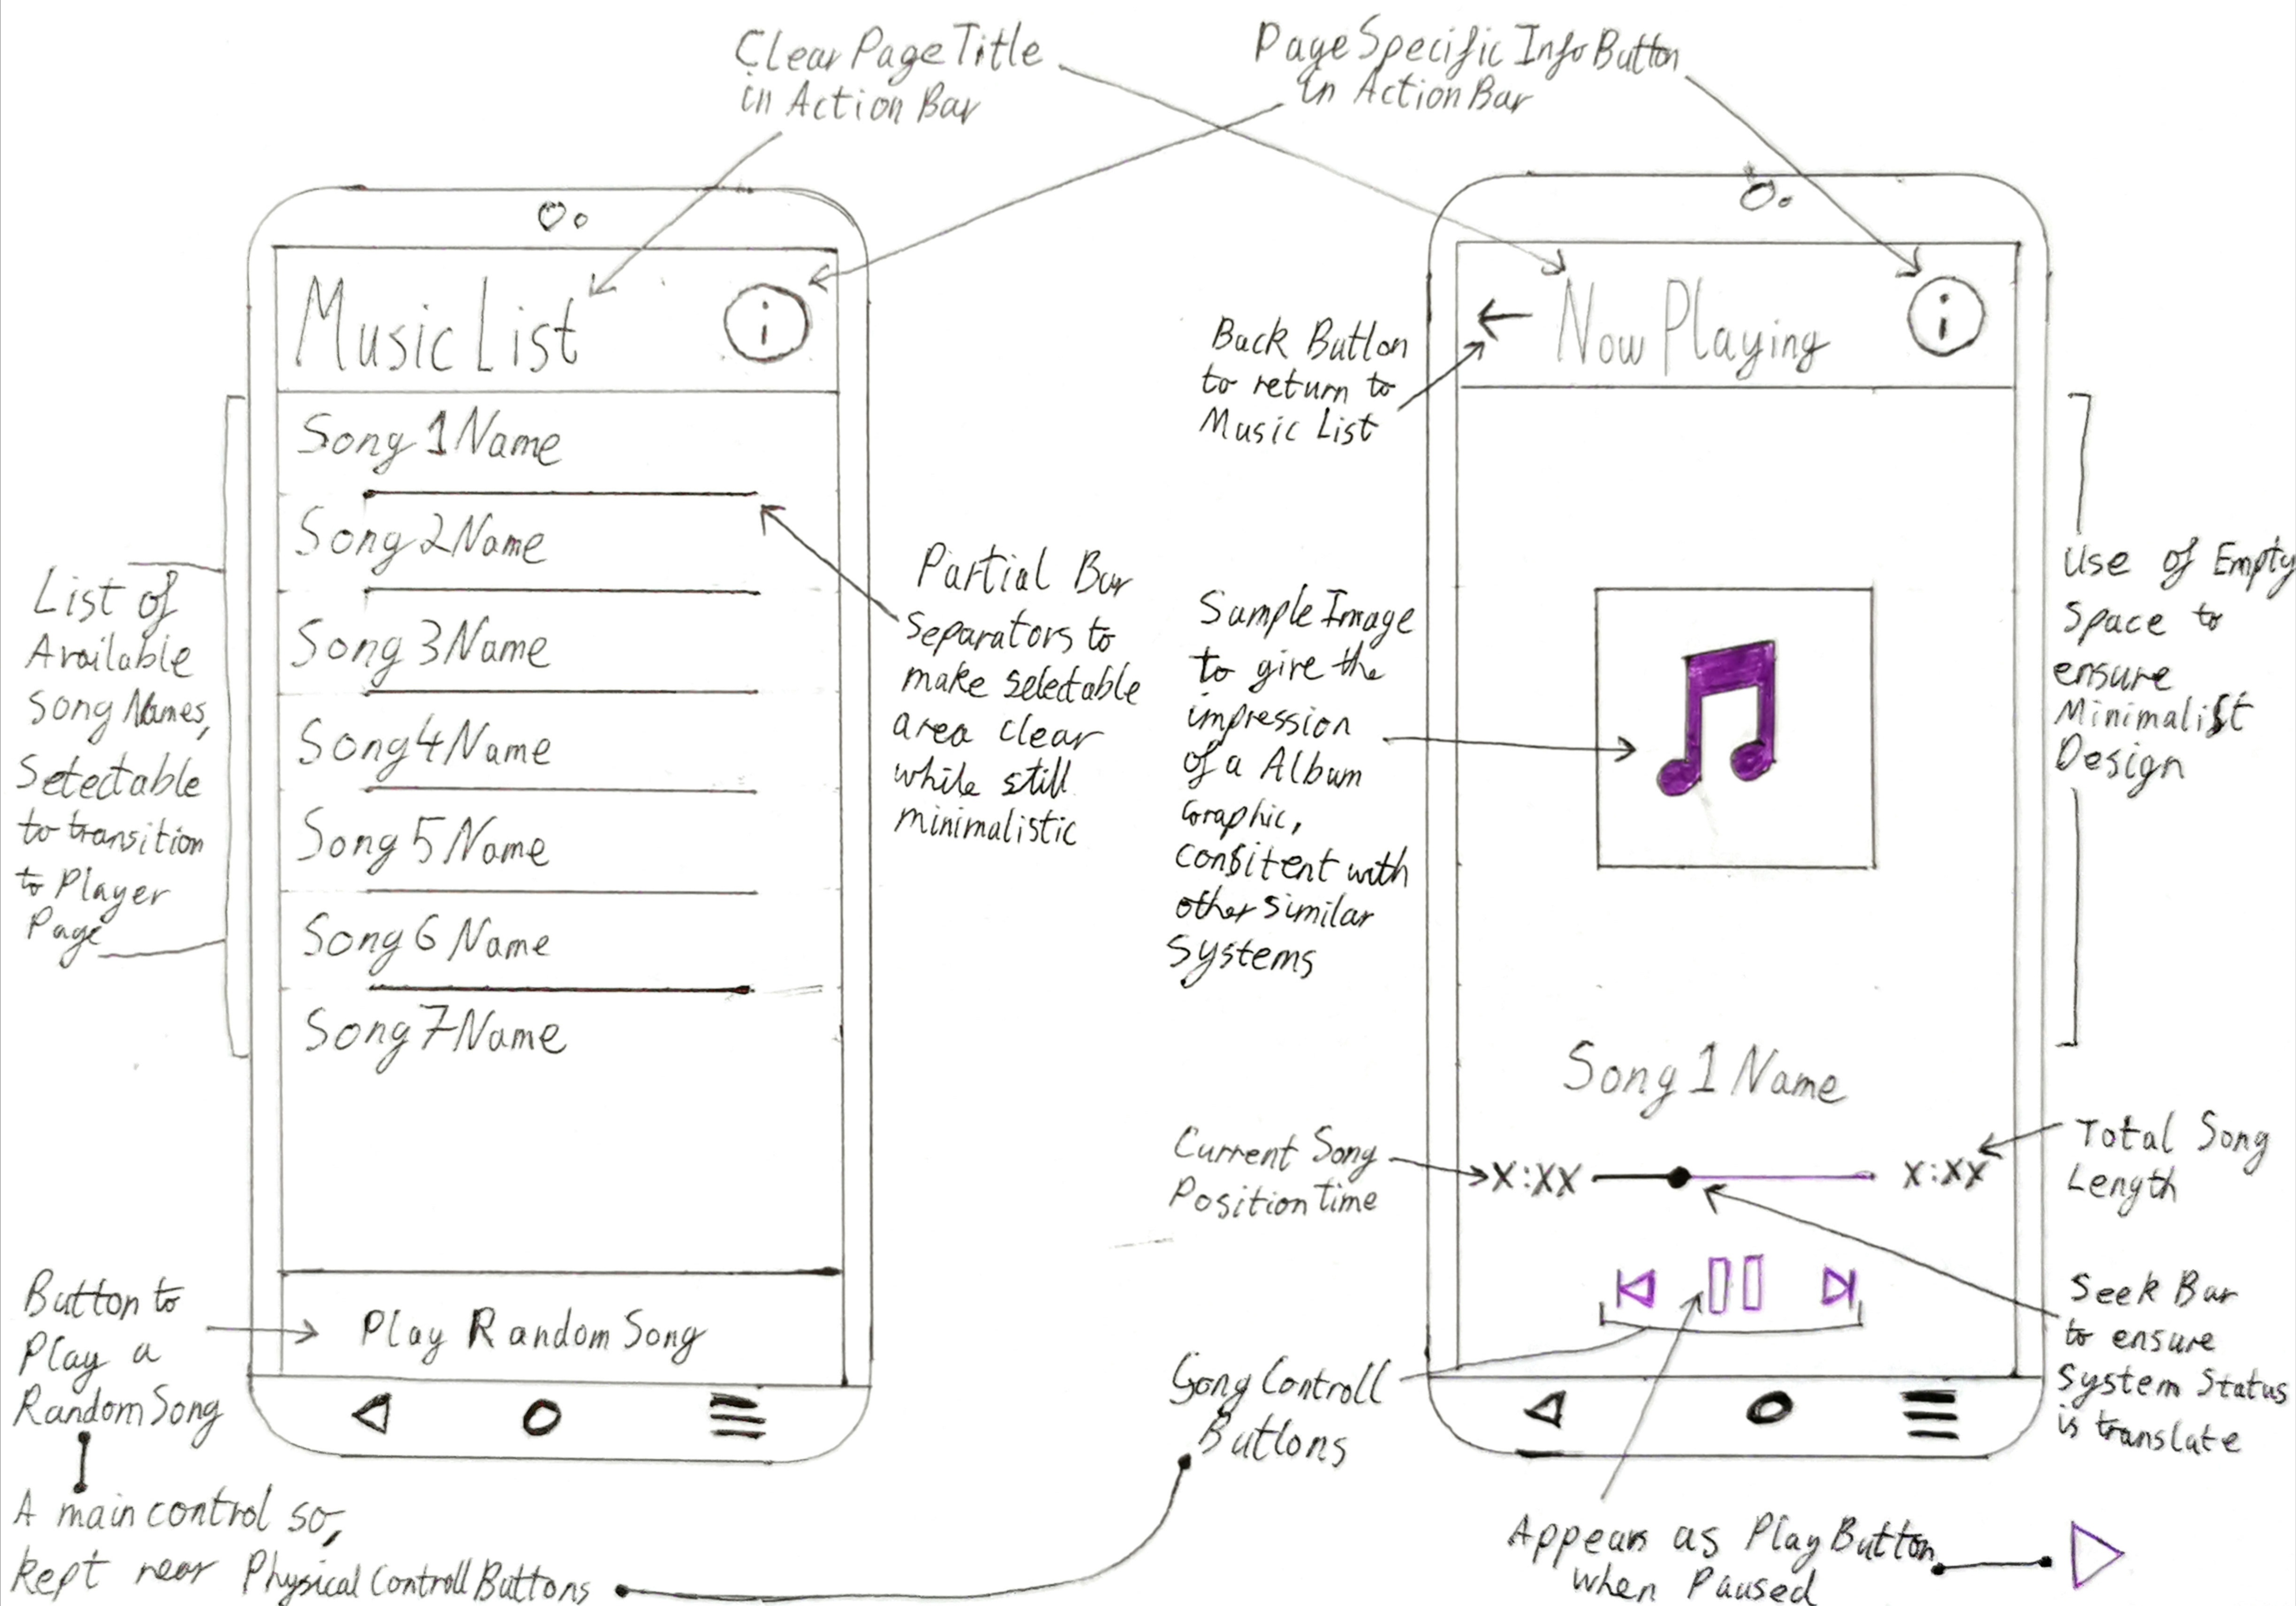
\includegraphics[width=\textwidth]{images/papWF.jpg}
        \caption{Paper wire-frames of the Song List and Player Pages, noting various design attributes and reasoning for them.}
        \label{fig:paperWF}
\end{figure}

Following the creation of paper wire frames, the 10 usability heuristics would be considered and the final prototype would be developed. Some examples are shown in Figure \ref{fig:digitalWF}. This stage between preliminary low fidelity wireframes and the final implementation is a crucial part of the process. The intermediate prototype gives a more detailed and realistic experience for how the application will function. When considering visibility of system status, the seek bar was included to ensure the status of the song that was playing was known to the user. The audible feedback of the song playing would also provide knowledge of system status to the user. A match between the system and the real world is met as icons for controlling the music are the same in design to ones used in physical audio player systems, also adhering to consistency and standards, and improving recognition rather than recall. Users have the control and freedom of when the audio will be playing with the various options on the player page. Users will also have control over what songs are available by simply downloading the songs they wish to their device. Only the file name and not the extension will be shown to ensure the user recognises the songs in the list. An aim of the gesture functionality is to increase the flexibility and efficiency of use. The flow of the pages was simplified, and the pages will have as little clutter as possible to ensure and aesthetic and minimalist design. Full lines between songs in the list were decided upon during the prototype development as partial lines looked cluttered and unfinished when viewed digitally and not on paper. When the calibration page was introduced during implementation, the error messages were designed to make the error recognisable, diagnosable and recoverable and info pages were directed to be for each individual page to ensure help and documentation was targeted and always accessible.

\begin{figure}[!htb]
    \centering
    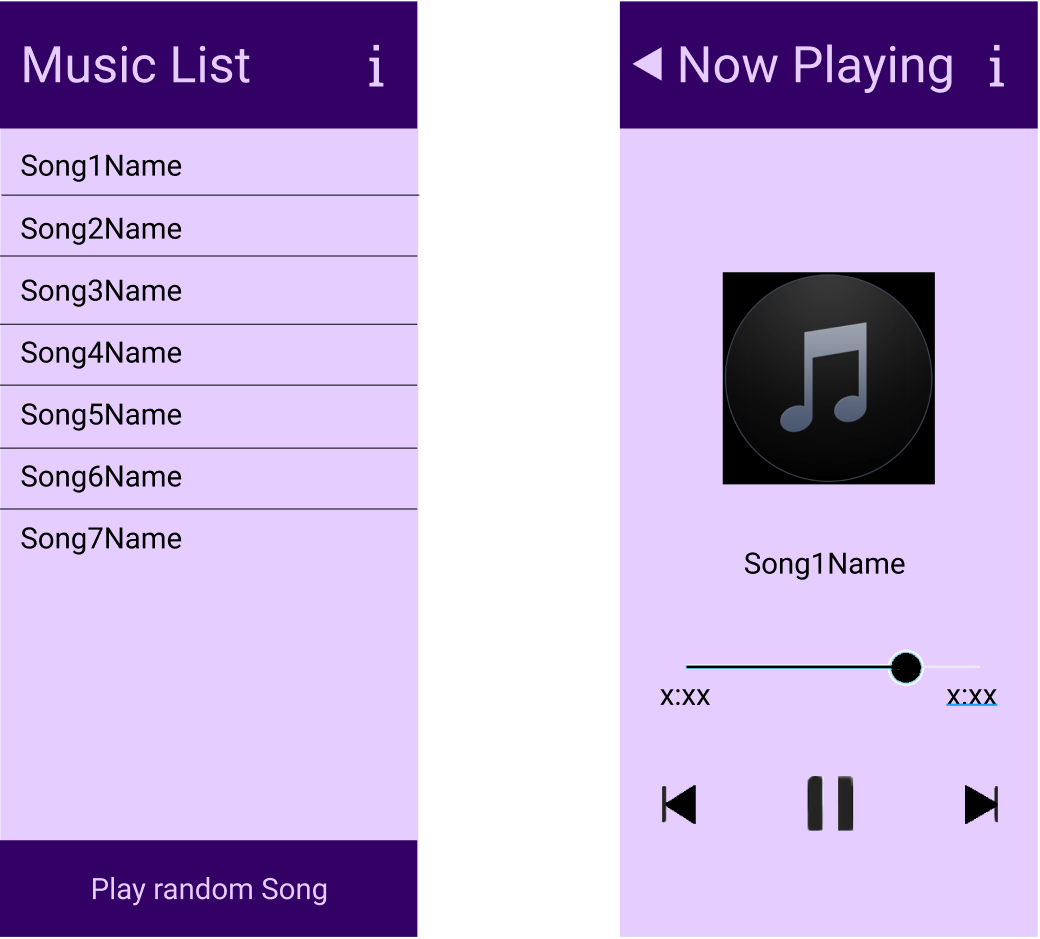
\includegraphics[width=0.75\textwidth]{images/DigWireframes.PNG}
        \caption{Digital wire-frames of the Song List and Player Pages, proving a detailed design and platform for exploring flow of the application}
        \label{fig:digitalWF}
\end{figure}

In addition to being used to enhance the applications adherence with the 10 usability heuristics. The flow and use cases were also explored. The platform in which the prototype was developed gave the opportunity to follow the flow of the application. Areas of the different pages can be encoded so that when clicked during the presentation view they will lead to other pages of the prototype. This allows the navigation's design to be be experimented with to ensure there are no issues and that all possibilities have been thought about before Implementation.

\subsection{Assets}

Due to the nature of the application being an audio player, it would obviously be redundant if the participants did not have access to audio files. Before time was wasted designing and developing a system without these assets, it was first confirmed that they could be gathered. It must be assumed that the participants do not already have these available and all assets must be made available with the software to ensure it is usable. These assets has originally been planned to be downloadable as part of the application file system package. However, the decision was made to alter this during development. The reasoning for this was that the implementation would read files from the user’s device to aid in customizability. It would also mean participants would not need to have the audio files on their device if they did not want them. This could use up valuable storage space on the user’s device unnecessarily. 

This change of path inferred that audio files would need to be made available for users in a different manner. Audio files were sourced using ccMixter. These files and the appropriate references of creators to be credited were made available to download separately from the application. Users were given the choice to download these files if they so pleased, however this was not necessary if they had their own audio files already downloaded to their device. In important step in this process was ensuring there was no breaches of any laws. All music files that were made available to download were sourced from a website that promoted the downloading and altering of audio files while adhering to creative commons. All documentation and relevant credits to the creators, contributors, and musicians.

Various images and icons were used throughout the implementation of the application. To avoid the need to credit the source of any images, the background image used throughout the development was personally created digitally. The icons used as various buttons throughout the app are provided as vector images by the Android Studio Software Integrated Development Environment.


\subsection{Gestures}

Gestures were carefully chosen to be the novel interaction technique that would be evaluated. Two gestures would be implemented for different functions. These functions would be pre-existing within the application and would ordinarily be activated by pressing a button on the touch screen. The gestures would provide alternative means to activate these features. State diagrams were initially used to consider the design of the gestures. A particular focus of this was to decide when and how the system would detect and react to gestures and what the consequences would be on different situations. 

The first gesture was chosen to be a Mid-Air Gesture. The function was to pause the music if it was currently playing or to start playing music again if it had previously been paused. This Gesture could only be accessed when the Player activity was active. The gesture would be activated by holding a hand up to the front of the device, around an inch away from it. This was chosen at it may be familiar to the users to being similar to a stop hand signal. 

This gesture was initially implemented by measuring the ambient light sensor on the mobile device and if it became substantially lower it would detect this as the hand being held over it. However, it was later found that the light level in the location it was being attempted. For example, if it was being performed in a dark place it would not detect a decrease in light. It was then decided that using the proximity sensor in the device was more adequate. This would ensure external light levels would not be a hindrance on performance. During implementation, the Sensor class was used to enable the app to detect this on a SensorEvent. The initial values were not checked to see if a gesture was detected to ensure errors were prevented. The first set of values will not have anything to be compared t. The stream of data was read and if the proximity value changed so that the current value was less than 80\% of the previous value the play/pause button would be activated, as shown in Algorithm \ref{lst:Proximity}. This threshold value was determined through various testing to ensure it was adequate. This gesture could not again be activated until the initial instance was complete and the hand was moved away.

\begin{lstlisting}[language=python, float, caption={Java code detailing how the Pause/Play Gesture is detected and how it is acted upon.}, label=lst:Proximity]

proximity.setListener(new Proximity.Listener() {
    @Override
    public void onRotation(float prox) {
        # ensure first passed is not checked for a change to ensure there is a previous value to compare to
        if (!firstProx) {
            # Check if gesture has been detected
            if (prox < lastProx * 0.8) {
                If so perform gesture function
                pause.performClick();
                # ensure next iteration is missed
                firstProx = true;
            }
        # Dictate if it is the first pass
        } else { firstProx = false; }
        lastProx = prox;
    }
});
\end{lstlisting}

The other gesture that was chosen would be of a Device Motion style. The function of which was to begin playing a random song from the list. This gesture could be performed when either the Tunes or the Player activity was active. The gesture would be performed by simply shaking the device. This was chosen as a suitable action as it mimicked the motion of rolling some dice to give a random number, in this case a random song. When on the Tunes List page this would simply activate a button press on the random song button which would generate a random number with a maximum equal to the number of songs available. The song in this position would them be selected. When on the Player page and the gesture is detected it will generate a random number with a maximum equal to the number of songs available. However, in this instance it would call the skip button but with the argument of the random number, intending to skip that many places in the list and play the equivalent song.

This gesture was implemented by measuring the changes in the device's accelerometers three axis. If there was a notable increase, then it would be detected as this gesture being performed. The accelerometer data stream was gathered again by making use of the SensorEvent values. The accelerometer would provide 3 values, the acceleration force along each of the x, y and z axis. This would factor in the force exerted by gravity. Following the previous gesture, the initial values from the were not checked to see if a gesture was detected to ensure errors were prevented as the first set of values will not have anything to be compared to. The gesture was detected in the difference between the current value and the previous value in at least 2 axis was found to be greater than a threshold value, as shown in Algorithm \ref{lst:Accelerometer} . Only 2 axis were required to mee this threshold as it was found that when shaking a device this if often only moved substantially in 2 axis with the acceleration of the third staying low. If all three were required to meet the threshold this would become very difficult for users to complete. The threshold was determined at the calibration step when the app is initially opened.

\begin{lstlisting}[language=python, float, caption={Java code detailing how the Shake Gesture is detected and how it is acted upon, this particular instance for when detection is made on the Tunes Activity.}, label=lst:Accelerometer]
accelerometer.setListener(new Accelerometer.Listener() {
    @Override
    public void onTranslation(float currX, float currY, float currZ) {
        # Ensure first pass is missed to ensure lastX, lastY and lastZ have values
        # There must also be songs available 
        if(!accFirst && loaded) {
            xDiff = Math.abs(lastX - currX);
            yDiff = Math.abs(lastY - currY);
            zDiff = Math.abs(lastZ - currZ);

            # Calculate if change is higher that the htreshold in any two axis
            if ((xDiff > threshH && yDiff > threshH) || (xDiff > threshH && zDiff > threshH) || (yDiff > threshH && zDiff > threshH)){
                # 
                shuffle.performClick();
                accFirst = true;
            }
        # Dictate if it is the first pass
        }else {accFirst = false;}

        # Set the current values to be compared against n next iteration
        lastX = currX;
        lastY = currY;
        lastZ = currZ;
    }        
});
\end{lstlisting}

A simple constant integer for this threshold value was initially used. However, during testing it was found that different devices would require different threshold values. It is thought that this could be due to the sensitivity of the hardware sensors in specific devices. It was at this point it became necessary to include the calibration on opening the application. Doing this ensured error prevention and usability of the gesture over all devices. The user is asked to shake their device and the accelerometer values are read at this point. The average of each of the highest values for each axis during this time is then calculated and taken to be the threshold value, as shown in Algorithm\ref{lst:Calibrator}. This makes the gesture far more reliable with the minor inconvenience to the user when they start the application. The user will only be allowed to proceed from the calibration page if there is some movement detected, ensuring they have actually shaken the device purposefully. If the threshold is not set accordingly for the user, they have the option to re-calibrate.

\begin{lstlisting}[language=python, float, caption={Java Code used to implement the Calibration stage on opening the application. Showing how the shake gesture threshold is calculated and how this step is enforced.}, label=lst:Calibrator]
protected void onCreate(@Nullable Bundle savedInstanceState) {
    super.onCreate(savedInstanceState);
    setContentView(R.layout.calibrate_acc);
    getSupportActionBar().setTitle("Calibrate");

    # Review accelerometer data and calculate the threshold
    accelerometer = new Accelerometer( this);
    accelerometer.setListener(new Accelerometer.Listener() {
        @Override
        public void onTranslation(float currX, float currY, float currZ) {
            # Ensure first pass is missed to ensure initial values are not compared
            if(!accFirst) {
                if (currX > maxX) { maxX = currX; }
                if (currY > maxY) { maxY = currY; }
                if (currZ > maxZ) { maxZ = currZ; }
                MAX = (float) ((maxX+maxY+maxZ)/3);
            }else {accFirst = false;}
        }
    });

    # Calibrate button function
    calibrate = findViewById(R.id.calibrate);
    calibrate.setOnClickListener(new View.OnClickListener() {
        @Override
        public void onClick(View v) {
            # Decide if phone has been shaken
            if (MAX > 0.5){
                # if so then start next activity
                openActivity(MAX);
            # If phone has not been shaken the show toast 
            } else {Toast.makeText(getApplicationContext(),"Please Shake",Toast.LENGTH_SHORT).show();}
        }
    });
}
\end{lstlisting}

\subsection{Implementation}

Following the planning, gathering of assets, and designing of the application, programming implementation commenced. All implementation was done in an Android studio using Java and kept under version control on GitLab --- local backups were also kept both on my personal machine and a USB flash drive. Initially a simple app to change the colour of the screen by doing various gestures was created. This was simply to gain and understanding of the potential uses of the hardware sensors and to confirm that it was possible for the chosen gestures to be detected. Following this, a music player app was created in which to build the gesture functionality upon. Finally, the gestures were then implemented to adhere to the context of the music player application.

An activity was first created to show a list of all .mp3 or .wav files on the device, the Tunes Activity. This was done by searching the device storage for files ending with .mp3 or .wav at the top file hierarchy of the device storage and then recursively check this for each subsequent child folder until storage has been checked. To do this it was required that the user granted permission to the application to access its storage. If this was not granted, then it was not done, and the user was informed of the consequences of this and directed to how permission can be changed to be granted.

Following this, a second activity was created to be the Player page. When any song on the list on the Tunes activity is selected, this would initiate the Player activity and begin playing that song. Buttons were created on this page to allow the user to pause the music if it was playing, play it again if it had been paused, these buttons were placed in the same position with the intention of only making them visible and press-able when adequate. For example, if the music was already paused, the pause button would net be shown and unable to be pressed. Buttons were also added to skip to the next song in the list and play the previous song in the list. It the current song was at the end of the list; it would loop back round to the first in the list if the next button was pressed. The same goes for if the prev button is pressed when the current song is first in the list. The file name was also shown in the is page. It was decided that the file type (.mp3 or .wav) would again be stripped from the end to make it more recognisable to the user. The text also moved across the page if it was too long to fit to ensure the user would be able to read the full name. The user had the option to go back to the Tunes activity using the back button in the action bar. Finally, a button to play a random song in the list was implemented to be fixed at the bottom of the Tunes view. This would generate a random number with a maximum equal to the number of songs available. The song in this position of the list would them be selected and it would begin playing.

There was a seek bar to be implemented on the Player activity in an attempt to give users more control and for them to have a better understanding of system status. However, during testing, many issues were found when the song finished it is a song was skipped. There seemed to be no consistencies to when it worked correctly and when it did not. Much time was spent in an attempt to fix this, but the root cause could not be found. At this time, the decision was taken to remove this feature as it was not an integral feature of the system. Additionally, if not all bugs were found in it then it could become a distraction to the user, and they may lose confidence in the application and create bias results that are skewed.

Various methods to implement the audio playing feature were considered. The two that were focused upon were (1)~The Android MediaPlayer APIs or, (2)~The Spotify SDK. Android Media Player provided the possibility to play audio files from the user’s device, files in the applications file system or from a data stream over a network. This gave flexibility of how the audio files would be provided to users while also remaining stand alone and non-reliant on other systems. Using the Spotify SDK would infer a reliance on the user having access to Spotify and depend on the Spotify application working correctly. This means there could be issues with different types of Spotify accounts, shared accounts and also narrow the potential participants as some people may not use Spotify. It would also infer that if for some reason the users Spotify app were to fail then the application would also cease to run smoothly, giving the participant a negative bias towards the app and skewing the results. For this reason, it was decided to use the Android MediaPlayer API. The aim was originally to embed the audio files within the application file system, but this was later changed to read files from the user’s device. This allowed users to listen to their pre-existing music already on their device and not have to use the music supplied. This was decided as it gave the user more freedom and customization, increasing the usability heuristics of the application and reducing external factors that may affect results gathered from participants.

Once it was decided that the Music Player system was completed the Gesture interaction capabilities were added to the application. Light Detector and Accelerometer classes were created to access and handle the data from the sensors to then be used by the other activities to decide what happens when a gesture is detected. Do be able to use this data and these sensors the user needed to be asked to provide permission to do this. How gesture detection was decided is detailed in the Gestures Section...ref to gesture --- . Information buttons were added to the action bar on each of the pages. This would spring a pop-up box, detailing what gestures were possible to do on each of the pages. Images were also shown on the popup do demonstrate how to perform the gesture. These could be exited by tapping anywhere outside the box.

Following the initial testing of the Mid-Air gesture, it was found that it was not reliable. In this case it was due to the nature of the light sensor. If there was very little ambient light in the room, the light level when no gesture was being completed was very low. The intention was that when a significant change occurred in the light level then it would be assumed that the gesture was being performed. However, this low level in the ambient state meant that when the gesture was being performed not a large enough change was being detected. However, this could not simply be amended by lowering the threshold of change that was required as other changes in light level were also having an effect. For example, if there was a light on in the room that was turned off, a significant change was detected, and it accepted this is the gesture being performed when it was not. It was decided that too many external factors were interfering with the light sensor. To counter these issues, the fix was to instead use the proximity sensor. It was originally not used as it was thought the user may need to get too close to it but after it had been implemented in the same way as the other sensor detectors it was found to be very efficient.

After testing, a calibration step was required for the shake gesture. This was implemented by creating an activity that the user would be met with upon opening the application. The user would be directed to shake the device and then press a calibrate button. When the user shakes the device, the accelerometer data is read, and a sample shake threshold is found by the sample gesture the used performs. This is used as a value to detect further shake gestures the user will perform while using the main functionalities of the application. To ensure this calibration is controllable, an additional button was added to the action bar. This can be accessed by the user from anywhere on the application and will return them to the calibration step in the case that they have not performed the gesture in an ideal way on the previous calibration attempt.

Another issue was encountered when first attempting to create the music player portion of the application. There was a requirement that the Android Studio platform was to be updated. In doing so, there were parts of the project gradle that seemed to be altered. This meant that the project could not build appropriately and could not be tested or used. This was an immediate issue that needed to be resolved. An attempt was made to revert this change within Android studio, but to no avail. Following this manual changes to the gradle files were attempted but again there was no success. The inevitable solution was to revert to a previous version that was pushed to the Git Repository. It appeared that the most recent version had the same issue, so the second most recent version was used. This was a timely set back as time was taken in an attempt to fix the issue. Time was also taken to catch up to the point that was reached before the issue was encountered due to having to pull a version from the Git Repository that was not the most up to date. It was at this point that physical backups were also made to ensure this problem, or any similar issue, did not arise again.


\section{Testing}

Testing of the application was done in three general stages throughout the implementation. Android Studio provides the opportunity to run the application that has been created on an android mobile device emulator. This was used for the majority of the testing at the stage of creating and completing the music player. Following this, the gesture detection was completed, and the thresholds were then tested using a single personal device. Finally, the application was tested over numerous devices from a range of manufacturers and production dates to unsure full functionality for all potential users. Throughout the process the debug function provided by Android Studio was utilised.

The aim of the first stage coding development was to produce a music player application in which the gesture capabilities would then be built upon. It needed to be confirmed that this portion of the application was fully functioning and without bugs or errors. As each component was added to the base activities, they were tested using the Android Virtual Device facilities in Android Studio. In this instance a virtual Google Pixel 3a was used. This provided a means of running the application in a safe space without having to download and install it on a physical device. 

If access to storage and sensors were accepted, then all audio files appeared correctly on the Tunes Page. However, if it was only temporarily denied --- not permanently --- the next time opening the app would act as though it was permanently denied and would not again ask for permission. This was decided to not be user friendly as if the user decided that they did then want to grant permission, this could not be done through the application. To fix this issue the code was amended to always ask for permission unless it had previously been granted or to always be denied. When selected, the songs played properly, as did the play/pause button. However, when the prev/skip buttons were pressed when the music was paused it should begin playing again. It did this but the status of the pause/play button did not change as expected and the code needed to be altered. It was found that if a song was allowed to run to the end, the next song did not play which was fixed through the addition of an onCompletion listener that would activate the skip button when a song finished so that the next one played. There was a further issue with this as the file extension was shown in the song name when this happened which needed to be amended as users would not expect this to happen and possibly gain a negative outlook on the quality of the application. The back button to return to navigate back to the Tunes page worked correctly and the music continued to play as expected. It was found that the random song button also acted as expected for the set songs that were added to the AVDs storage. At this point it was decided that the music player was working to the standard that was aimed towards.


During the addition of the gesture detection capabilities the functionalities were examined using a single personal device. It was decided that at this point it was no longer viable to test the application using the AVD as the sensors on the virtual device were not accurately controllable. Using the Android Studio IDE meant that the application could quickly be deployed to the device using a wired connection to build and install the current version of the application.

On opening the application, all permissions were handles correctly and as expected. When viewing the audio files that were gathered from storage, files from other applications that were not conceptually intended pleasurable music listening were included (e.g., ringtones and sound effects). This was countered by adding checks and restrictions to the names of the files that were being retrieved and made available. The information icon on the action bar was found to be too large so was reduced in size. The shaking gesture was not detected so the constant threshold value was reduced to an appropriate value. Once this had been achieved, a random song started when viewing either the Tunes or Player Activities were active and shaking the device the appropriate amount, as expected. Edge cases were tasted by moving the device in ways that would be presumed natural and ensuring that it was not registered as gesture. As previously stated, the Light Detector that had been implemented at this point was found to be fundamentally flawed. Inferring the gesture unusable and other options were explored. This was found by moving the phone naturally through multiple environments and attempting the gesture to try to find edge cases for registering the gesture. The alternative that was decided upon was to amend the implementation to use the proximity sensor in its place. This was found to be much more reliable than the Light Detector. Music was successfully paused and played when the gesture was detected. This only happened when the Player Activity was active, as expected.

When it was decided that the application worked adequately for the individual device, the next step was to ensure that the application could be downloaded remotely to other devices. It also was required to work in the same way on these other devices as it did on the first. It was originally presumed that this would be a given situation, however this was not the case.


When downloading to devices remotely, devices ranging from a production date from 2016 to 2020 and from a variety of manufacturers. this was done to ensure that it was understood how the application could be distributed. After various trial and error attempts using various methods, various potential and effective ways of installation were found. Once installation was complete the same test as above were completed, and response was successful with the following exceptions. There was one more set of unwanted files on the displayed list which were dealt with in the same manner as previously. It was assumed that this covered almost all instances as no participants were found to have any unwanted audio files in the list on the application. the other Issue that was found was more substantial. On various devices the shake gesture was too easily detected, requiring almost no motion at all, while others were unable to detect the gesture unless the device was very vigorously shaken. The reason for this is thought to be due to the sensitivity of the sensors used by different manufacturers. Devices from common manufacturers required the save vigour of shaking. Some research was done to confirm this. To combat this, the previously mentioned calibration step was introduced.

Following the addition of the Calibration set it again required testing. As before it was first adjusted to adhere to an individual device, followed by a wider pilot. This additional activity required permission to be granted earlier in the app’s usage. This was tested by opening the app and noting when the permission was requested, it performed as expected. The calibration was tested first by shaking he device a normal amount during calibration and then attempting to perform the gesture with as similar motion as possible to ensure it worked accordingly which it did. An additional test involved attempting to calibrate the device without shaking it to ensure this was not allowed and the toast appeared, which it did. A further test was to ensure that if during calibration the shake was too vigorous, and the gesture was then too difficult to perform, that the user had the option to re-calibrate. This was possible through the addition on a re-calibrate button in the action bar which was available anywhere on the app. This button initiated a popup ensuring the user knew that this was what was about to happen. If they accepted, this successfully allowed the user to return to the calibration step. It was not accepted by the user, the popup disappeared, and the current calibration was maintained allowing the user to continue using the application.

%==================================================================================================================================

\chapter{User Study}

\section{Outline}
Participants would experience using a novel interaction technique, that they had little familiarity of using previously. In this case, it was decided that the novel interaction technique in question would be Device Motion Gestures and Mid-Air Gestures. This technique would be made available to them on their personal mobile device. Ensuring the user is familiar with the environment in which the interaction technique is built upon is very important to ensure no other external factors on unfamiliarity infer secondary effect. Participants would be provided an information leaflet and a consent forms to complete in line with the ethics checklist. Participants would then be asked to complete surveys at a specific time frame during the experiment’s timeline. Collecting data throughout the experiment on the user’s experiences is important to understand opinions as time passes. Results were processed and searched for erroneous input, evidence of this was discarded from results. Statistical analysis was carried out using the Wilcoxon Rank Sum test and Results were analysed using other techniques. Results and their implications are discussed.

\section{Ethics}
Many ethical considerations were accounted for throughout this research. To meet common standards statd in the Department of Computing Science Ethics checklist form needed to be adhered to. This includes 12 main articles that should be met for all areas of the project. Particular care needed to be taken due to the Covid-19 pandemic. These requirements were also met during the requirements gathering survey.

Before any experimentation, participants were asked to read and complete a declaration of consent, This was done within the Google form survey for the requirements gathering survey. An overall declaration of consent for this User Study was provided to participants electronically, detailing the aims of the overall research and individual requirements form the participants at each stage. It was made clear that a participant could ask for more information at any stage as well as ask to be removed at any time, in which case all date that was held relating to them would be deleted and not used in the study. Users were asked to provide further consent for every individual survey throughout the User Study. Each of which detailing the same as the above with additional details of the aims that specific survey and how long they should expect to have to spend doing it. When the final survey was completed by the participant and the study had come to an end, they were provided with an experiment debrief, containing information about what would be done with the data collected and how they could remain in communication in the case of any addition information they may require or if they wish to withdraw form the study. 

Upon commencing he research, each participant was supplied with an information leaflet. This would again detail the aims of the research along with the suspected timeline of the experiment and what would be required of the participant throughout. It provided information and instructions of how to prepare their device to run the application along with how to download and install the software required to take part. Information detailing how to use the application and its potential use cases were described to ensure the user was well informed at all times. 

Over the curse of the User study, participants are required to complete 4 different surveys, all on different days. This introduced the issue of data continuity. Participants responses to all the surveys needed to be coupled so that they could be compared over time. To do this, participants were asked to provide a pseudonym that would be provided at the start of all surveys to enable this to be done. To ensure anonymity participants were advised not make this their name, email, username, password, birthday, address or similar that may relate to them. It was recommended that they use a random word, number, sequence or other combination that they would be able to remember and supply throughout. Ensuring anonymity of these pseudonyms was of upmost importance to ensure that the participants were safe from any threats or dangers that could relate data back to them. Adhering to the intent of the ethics checklist was a priority.

\section{Method}
Following final testing of Motion Music and considering any ethical implications, participants were sought out under the following criteria. Participants were required to have an android device so to ensure that it would be possible to install and use the application. Participants needed to to have little experience using the types of gesture in question to ensure a level playing field for growing more used to the novel interaction technique. Participants need to cover a varying age range and technical knowledge to ensure that the sample is a proper representation of the population. To ensure these criteria were met a surplus of potential participants were asked to take part. All but 2 people that were asked to take part had an android phone reducing the potential sample size from 10 to 8, N = 8. All remaining participants had very little to no experience using these Gesture types in the past and covered the other set requirements.

Available participants were then asked to thoroughly read the declaration of consent and sign it. This is to ensure that the fully understand what is involved with taking part in the experiment and are happy that the data that they provide will be analysed and used to draw conclusions from. Participants were also asked to thoroughly read the information sheet that was provided to them to understand in detail what would happen at each stage of the process. This document detailed that an initial survey should be completed before the application would be installed to understand the users current perceptions of Gestures and reasons they feel they are or are not socially accepted. It asked the participant to say which type of gestures they believed they device to be able to recognise and how regularly they use each gesture type. They were asked to detail situations in which they would be happy to use one of these gestures if they had the option to use the touch screen for a required function and to detail situations in which they would be happy to use one of these gestures if they had no option to use the touch screen for a required function. The purpose of this was to gain a knowledge of just how much experience the participants had previously using the novel interaction techniques in question. It would also supply valuable knowledge of their base views on the gesture inputs that could then be compared to their vies throughout and after the process to see if they had changed.
Participants were the debriefed and directed to the next task.

After this initial survey before using the application, participants were asked to install the Motion Music application on their device. Instructions informing the participants of a way that this could be done were included in the information leaflet. However, most participants required some assistance to do this as it is fairly complicated. This was of course provided over instant messaging, phone call or video call ---whichever suited the participant. At this point Participants were also directed to download the music files of their choosing of the audio files sourced from ccMixter. They were encouraged to download a .txt file associated with each song with the appropriate reference and crediting to the creator. The participants were also informed that they did not need to do this if they had pre-existing music files saved to their device storage or they could choose to download audio files from another source.

Once each participant had installed Motion Music they were then directed as to how to use the application and when the following surveys should be completed. Users were asked to refer to the usage guide in the information leaflet. This portion of the leaflet informed the participant on how to complete the calibration step on opening the application, the functions it had and the various methods of implementing these functions --- through both the touch screen and gestures. This was done to ensure the participant understood the full potential of the application and were able to utilize all functions. It also meant that participants did not expect the application to do more than it was capable of as this may lead to frustration which could return bias results. Users were informed that a survey was to be completed after one day of using the application, after three days of using the application and after one week of using the application. These intervals were used to capture how users felt after briefly using the application, after using it for a short time and after a full average weekly schedule of the participants life. 

Participant progress was tracked over this time to ensure surveys were distributed and completed by the correct people at the correct time. This was important to keep consistency as some participants started the process at different times. Each of the surveys aimed to track how much the participant used the application and what their perceptions and opinions of the gestures were. The three surveys asked the participant the same questions with the exception of the final survey for use after a week. This survey had the same questions included with some additional question to allow the participant to reflect on the time they have used the application and gestures for.

The common questions over these three surveys gave the participant the opportunity to detail how many times they had used the application and each of the specific gestures. This was to understand how frequently they were using the application between surveys. This would eventually be compared to see if it had an effect on how quickly the participants got used to using the application. Users perceptions of how useful, how much effort was required to use and how socially acceptable each type of gesture was recorded in a Likert scale format. I Likert scale type question was also used to ask if they participant agreed, or not, that the gesture interactions felt gimmicky. The changes in users perceptions between surveys would be explored. Participants were asked to describe a time in which they thought that the gesture input was more useful for a situation as opposed to simply using the touch screen input alternative. They were asked this for each of the gesture types. Finally participants were asked to detail some comments on the system as a whole. Some examples were provided and users were asked which they agree with as well at the option to enter their own comments; I found the Gesture functions difficult to perform, I found it fairly hard to get in the way of using the Gesture functions, I consciously went out my way to try the Gesture functions, I tried to get better and more used to using the Gesture functions, I found myself using the Gesture functions without thinking about it. These qualitative views were tracked and compared throughout the process.

Finally, the survey for completion after a week of use was completed by participants to further delve into their experiences over the whole week of the process. participants were asked to determine which of the gestures they felt easiest to complete, most useful and which of the gestures they felt was socially acceptable in more circumstances. This was to supply a comparison of the participants gesture preferences. Paticipants were asked to rake on a Likert scale if they Agree, or not, that; they found themselves using the gestures without thinking about it, they  found the week eye opening to the potential gesture could have, they believe that mainstream applications don't currently and could make use of Device Motion and Mid-Air Gestures. This was to be used to compare the participants opinions on gesture use to what they previously thought about gestures before using the application. Participants were also asked if they had thought of a specific use gestures could have. This was asked to solidify their opinion on the potential gesture have.

Once all data had been collected, it was processed into an Excel spreadsheet in order to be analysed and evaluated. Likert scale data was ranked accordingly and plotted on graphs to better understand how participant views changed. Data sets of Likert scale data between the various surveys was also statistically analysed using the Wilcoxon rank sum test in order to determine of there was a significant difference in participant responses between the surveys. Themes in qualitative data were identified and patterns were found in order to draw conclusions.

\section{Results} 

As the participants progressed through their time experiencing the app and making use of the Gestures made available to them, they were providing data on their opinions through surveys. There responses were transferred to an Excel spreadsheet to be analysed. Before any analysis was carried out, the data was searched for any potential erroneous responses. Where possible these were amended accordingly or discarded where this was not possible. Where questions asked users to respond on a Likert scale, Strongly Agree was encoded to a rating of 5, Agree to 4, Neutral to 3, Disagree to 2 and Strongly Disagree to 1. This was done to better represent users responses numerically to be included in visualisations. Statistical analysis using the Wilcoxon Rank Sum test was then applied to these results to determine if there was a significant difference between the responses after one day of use to three days of use and between responses after three days of use to one week of use. This test was used as the data is in an interval fashion and a comparison across two groups ---two different time frames--- was required. This test provides a p-value, the probability of a null hypothesis, a significant difference being true when p-value $\leq{0.05}$ (5\%). The sample size was not as large as it could have been due to restrictions which was another reason this statistical analysis method was used. Users were required to supply an unidentifiable keyword used throughout to track their changes over time and ensure the correct data between surveys was coupled, while still ensuring anonymity throughout the results. 

\subsection{Usage changes}
All users use an android phone as their personal device so were used to the operating system the app was build for. None of the participants believed their device regularly gave them the option to use mid air gestures. 50\% knew their device to give them options to provide options for motion gestures and only 25\% had used this interaction method and it was said to be less than weekly use. If provided the option to use mid air or motion gestures, a quarter said they would continue just to use the touch screen option with all remaining participants detailing that it would depend on if the interaction would require less effort than simply using the touch screen, one of which said it would also depend on social situation. All participants that said they would continue to use the touch screen were the same participants that knew their device had motion gestures but didn't use them. When asked what they would do if a function required the use of Motion or Mid-Air Gestures, with NO touch screen alternative, 25\% said they would never use that function, 25\% said they would use it no matter what, simply because they wanted to use the function, one said they would use it if it suited the situation, one said they would use it if it was useful, one said they would use it if it took little effort to use and one said they would use it if it fitted the social situation but only if it was useful.

With exception of 1 participant, users  used the app 2-4 times or less after one day of use and again 2-4 further occasions after 3 days of use, with the exception of 2. Following this after one week, half the Participants used the app a further 5-10 times and the other half said they used it more than a further 10 times.This is easily visualised in Figure \ref{fig:usage} Users tended to use the Motion Gesture equal to or less than the amount of times they used the app, while using the mid air gesture equal to or more than the amount of times they used the app. One user asked after the survey for after 1 day of use if using the mid air gesture to pause and then play it again counted as one or two uses. After confirming that pausing an playing again only counted as one use of the feature due to its nature however if it was just use to pause or play and the button was used conversely it still counts as a use. This was then relayed to all other participants to confirm this was how they answered and would answer the usage questions in the surveys. Participants responded confirming that this is what they had assumed and answered all surveys accordingly.

\begin{figure}[!htb]
    \centering
    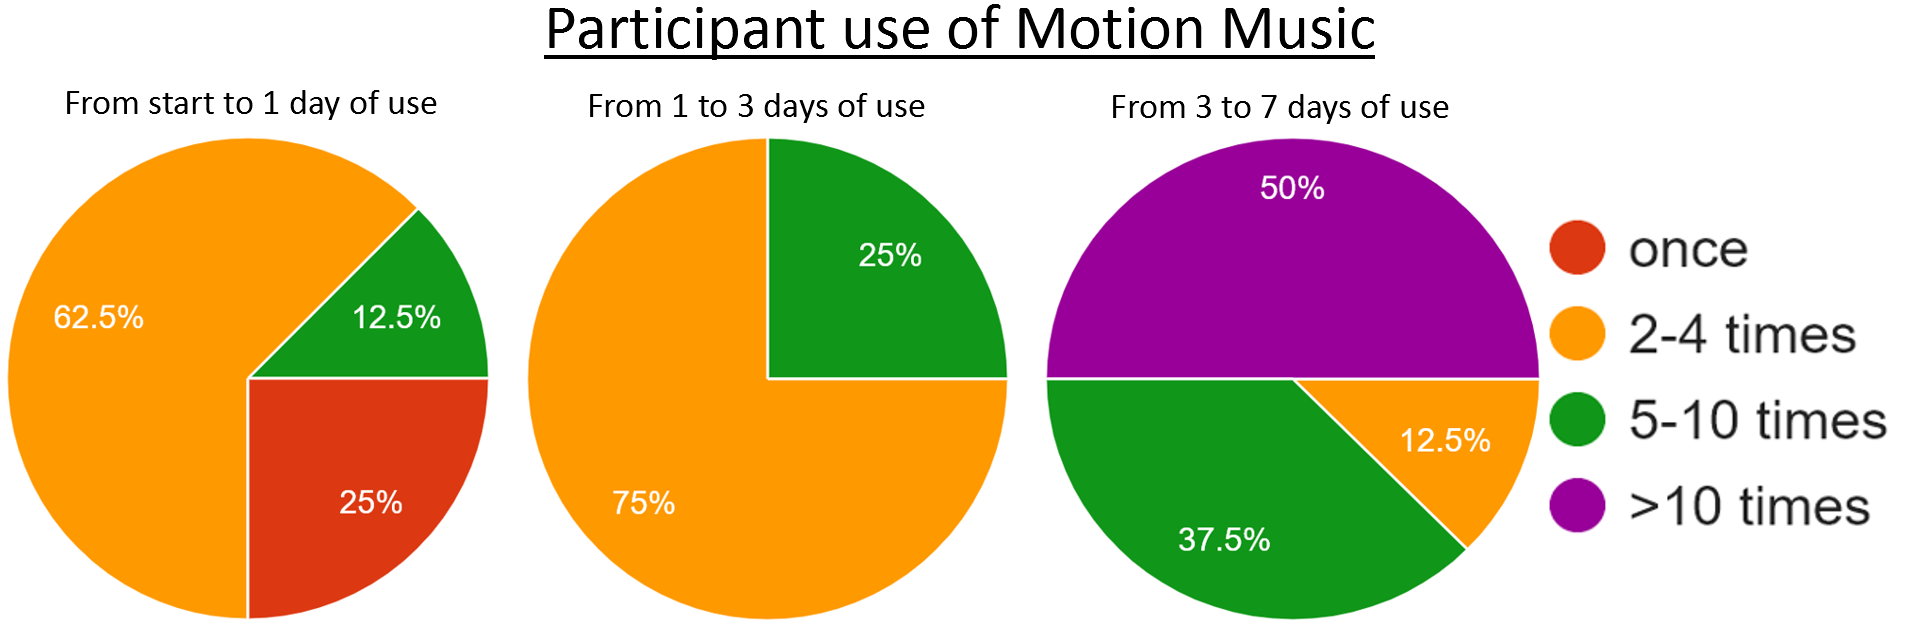
\includegraphics[width=\textwidth]{images/Use of MM.PNG}
        \caption{Pie charts showing the participants usage of the Motion Music application over one week. The left chart showing the usage after one day, the middle chart showing the usage between the first the third days use and the right chart showing usage from the third day of use until the end of the survey (one week use).}
        \label{fig:usage}
\end{figure}

\subsection{Participant Perceptions}

On average, after one day of use, participants rated the usefulness of both the Device Motion Gesture and the Mid Air Gesture Functions 2.25/5. This increased to 3.125 and 3.975 respectively after 3 days of use, the data sets giving a p-value of 0.008 and 0.019. After one week of use there was an increase to 4.25 and 4.375 respectively, with the data sets having p-values of 0.025 and 0.013. Increases can be seen on Figure \ref{fig:perceptions}. For the Device Motion gesture, after 3 days only half the participants were able to provide an example, however all were able to provide one after 1 week. For the Mid-air gesture, after 3 days all but one participant were able to provide an example, and again all were able to after a week.

The average rating of ease of use for the Device motion gesture had increased between 1 day and 3 days of use, from 2.125 to 3.875 and then to 4.5 after a week of use. The data sets providing a p-value of 0.19 and 0.23 respectively. The average rating of ease for the Mid-air gesture raised from 2.375 to 4 between 1 and 3 days of use and then to 4.875 after a week of use. The data sets providing p-values of 0.11 and 0.19 respectively. These changes can be visualised on Figure \ref{fig:perceptions}.

All participants either disagreed that the gestures were gimmicky or were neutral on the subject after 3 days of use, with data providing a p-value of 0.09 when responses were ranked from 1-5. 75\% of participants Strongly disagreed that the novel interaction techniques were gimmicky after a week of use, this change providing a p-value of 0.013. These responses were with respect to the the gesture interaction opportunities in general as opposed to a specific one of gestures available or with respect to the application as a whole.

Responses relating to perceived social acceptability were converted to values 1-5, 1 Strongly disagreeing that they would confidently use them in an unfamiliar locations or company and 5 Strongly Agreeing. There was increase from an average score of 2.5 to 3.5 for Device Motion gestures and 2.75 to 4 for Mid-Air Gestures form 1 day of use to 3. Data sets providing a p-value of 0.039 and 0.014 for Device Motion Gestures and Mid-Air Gestures respectively.No users disagreed that they would confidently use either gesture technique in unfamiliar company or location after only 3 days of use.  In the case of the Mid Air gesture, every participant strongly agreed that they would confidently use this novel interaction technique in unfamiliar company or an unfamiliar location after a week of use. After 7 days the average score was 4.375 for Device Motion gestures and 5 for Mid-Air gestures respectively. Data between 3 and 7 days providing p-values of 0.19 and 0.023 for Device Motion Gestures and Mid-Air Gestures respectively. Changes in participants confidence in using these gestures in unfamiliar locations or company can be visualised on Figure \ref{fig:perceptions}.

\begin{figure}[!htb]
    \centering
    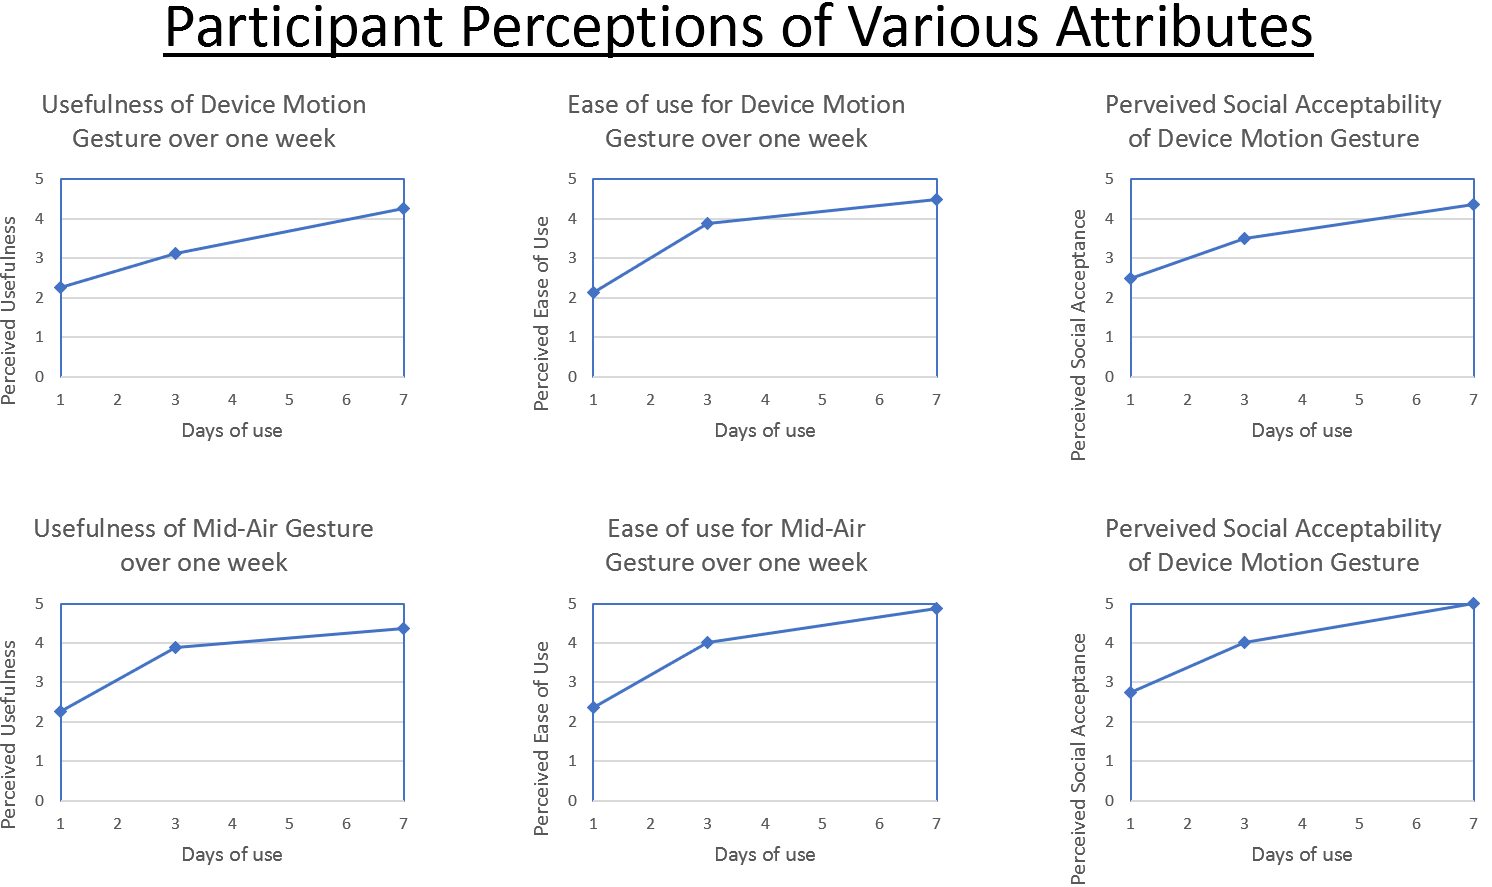
\includegraphics[width=\textwidth]{images/perceptions.PNG}
        \caption{Line Graphs showing the average participants responses for Usefulness(left column of graphs), Ease of Use(center column of graphs) and social acceptability(right column of graphs) for the Device Motion gestures(upper row) and Mid-Air gestures (lower Row).}
        \label{fig:perceptions}
\end{figure}

\subsection{Participant Opinions}
After one day of use, Five of the eight participants noted that they found it difficult to get used to using the gestures and those who did not were making the conscious decision to attempt to get in the way of using the gestures and get better at using them. After three days of use, 50\% noted that they were consciously going out their way to use the gestures, 25\% said they were trying to get better at using them and 25\% noted that they were using the gestures without thinking about it. Whereas, after a week of use, 5 of the eight participants strongly agreed that they had started us use the novel interaction techniques without consciously thinking about it and the remaining participants agreeing. All the participants strongly agreed that using the app over the week had made them more open to using these types of interaction in more social situations than they would have before using the app and/or believe that mainstream applications don't currently and could make use of Device Motion and Mid-Air Gestures.

At the end of the study, 75\% of participants noted that the felt the Mid-Air Gesture was easier than the Device Motion gesture and all but one participant thought the Mid-Air Gesture was more useful than the Device Motion gesture.

After a week of use, when asked to provide a circumstance where either gesture may not be acceptable, 75\% said that they may not use the device Motion Gesture in a cramped situation where it may result in physical contact with others or intruding in their personal spaces. One participant noted that they may not was to undertake exhaustive large movements when with their friends or in a meeting. One participant was unable to provide a circumstance. Only one participant was able to provide an example of when it may be unacceptable to use the Mid-Ar Gesture. They stated that it may seem a bit odd in the beginning but it would become more normal is time passed. Users were asked if they could provide any other functions where these types of gesture interactions could be implemented. Examples of these situations participants feel they may not use the gestures are listed in Figure \ref{fig:problems}. All participants responded with an example of an existing output with the gesture as an alternative way of controlling it, with half of the responses additionally providing reasoning that involved the gesture being used where the touch screen method of control used an excess of effort to complete. An example of this was to tilt to the side to remove all notifications as it can take time and effort to stretch to the top of the device to clear them all.

\begin{figure}[!htb]
    \centering
    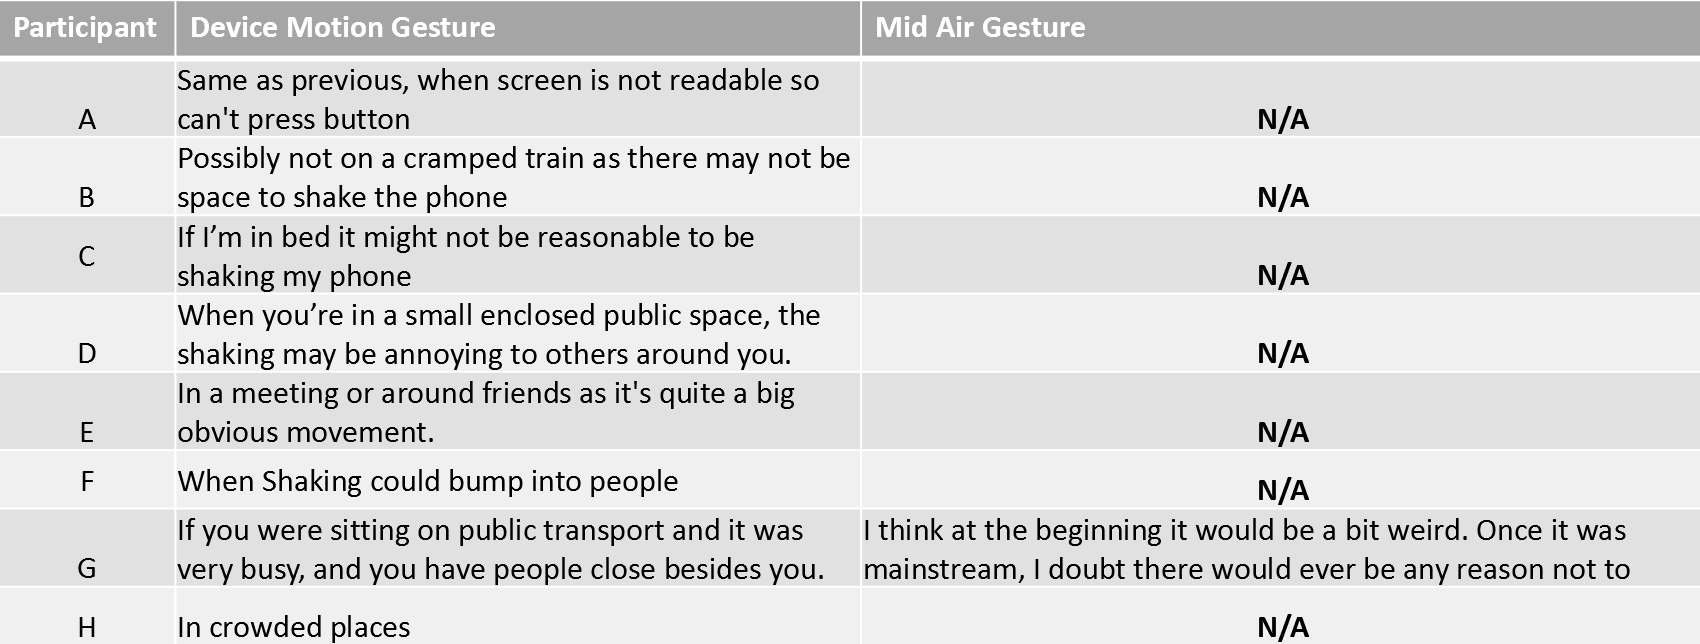
\includegraphics[width=\textwidth]{images/problems.PNG}
        \caption{Table detailing participant examples of then they might deem it socially unacceptable to use either type of gesture.}
        \label{fig:problems}
\end{figure}



\section{Discussion} 

\subsection{Usage change}

Participant usage of the application was fairly low over the first three days of use and increased significantly in the time after this until one week of use. Since \citet{zipf_human_2016} suggests that it is the social norm that a person will strive to expend the least amount of energy to solve a problem and accomplish a goal. Since towards the end of the week of use participants are more frequently using the application, it can be taken that the more frequently perceive the task of using the application as a whole to be more acceptable to complete, either due to finding the outcome of using the application as more valuable or less effort being required to use. 

At no point during the study did a participant say that they had use the Device Motion Gesture more times than they used the application. This is thought to be the case due to the nature of the function, one may not know what song to start with so play a random one but once the music had started the function was no longer required. However towards the end it became closer to the same amount of occurrences, meaning they may have used the function every time they used the application. The use of the Mid-Air Gesture function per use of the application also increased as the study went on, but this time the uses of the gesture exceeded the number of app uses. This it thought to be due to the demand for the output of this task being more frequent. The natural frequency of the need for the Mid-Air gestures result was higher than the need for the Device Motion Gestures result.


\subsection{Participant Perceptions}

Results showed that the increase of users perception of usefulness for the Device Motion Gestures was gradual over a week of use, yet between 1 day and 3 days of use for the Mid Air Gestures there was a significant initial increase compared to the rest of the period. This closely correlates to when users were able to provide an occasion in which they thought using the novel interaction was more useful or less effort than simply pressing the tough screen. Users provided circumstances for these questions when the effort to use the touchscreen was increased, for example when cooking and its likely you would need to wash your hands first so the screen didn't get dirty. In this instance the cover gesture required no contact so did not infer the added step of washing of hands. This meant that in this instance the gesture was particularly useful to the user. It can be taken from this that users perception of usefulness of a gesture considerably increased when they come across specific instances in which it was more useful than simply using the touch screen. Particularly when using the touchscreen was made more difficult than normal and the gesture seemed easier in comparison. As hypothesised, people will come across more more useful functions as time passes that were not evident before use, increasing the value they will get by using it. This is indicative that gestures should be considered as an alternative method to functions that are generally controlled by the touchscreen but may have common occurrences where this may be more difficult to use or where additional steps are required. These occurrences have been found to be when the users is moving and precision touch screen touches cannot be made or where an additional task is being undertaken in parallel to interacting with the device and the users attention is divided, for example cooking or driving. This will ensure that users will adhere to social norms of least effort as extra effort will not need to be used to use the touch screen in these difficult situations.

Users Perceptions of how gimmicky the gestures were were significantly changed over the course of the study. After one day of use, none of the participants disagreed or strongly disagreed that the gestures available on the application were gimmicky. However, after only one week of using the gestures on the application, all the participants disagreed or strongly disagreed that they were gimmicky. After becoming more aware to the potential uses of the gestures participants did not see them as contrived at all. This firmly backs up that the users felt that the gestures genuinely benefited the application and they weren't just available to be eye catching and fun. They believed they fitted well in the context of the application and did not lack real substance and value. It can be assumed that users found the gestures fitting for general use and therefore have a good level of perceived social acceptance.

The finding of new uses did not so closely correspond to the perceived ease of use in the same way that the usefulness factor did.The increase of ease of use in device motion and mid air gestures increases more rapidly at the beginning of the experiment than towards the end of the experiment. Both sets of data are more statistically different between 1 and 3 days of use than between 3 and 7 days of use. This is particularly significant since there was more time between 3 and 7 days of use to become more used to the gestures than there was between 1 and 3 days of use. Participant usage was much higher between 3 and 7 days. This indicates that the ease of use of a novel interaction technique that a user does not have a great deal of experience using becomes easy to use after as little as three days. This continues to require less effort to use until almost all participants strongly agreed that it took little to no effort to use mid air-gestures. It can be said that the more a person uses a new interaction method, they will become more used to using it and feel as though the desired outcome requires less effort and becomes more useful to them for accomplishing a task --- as hypothesised.

As time passed in the study, data collected showed that there was a strong suggestion that the usefulness off both gesture types increase drastically and the effort required to use the gestures decreases drastically, particularly in the first 3 days. There is also a significant increase in participants perception of the gestures social acceptability between 1 and 3 days and 3 and 7 days of use. Confirming the hypothesis that participants will find the gesture interactions more useful and easier to use over time, and in turn it will be perceived to be socially acceptable to use in more situations. This is particularly interesting as after such a short period of time of using the application, users views on how comfortable they would be using the gestures in an unfamiliar location or in front of an unfamiliar audience had drastically changed. These are the factors that many other studies \citep{rico_usable_2010, freeman_rhythmic_2017, ahlstrom_are_2014} had determined to large factors affecting social acceptability. In this case only a few days of becoming familiar with gestures has completely changed users views on using them in these previously thought to be unacceptable circumstances. When designing gestures and other novel interaction techniques, there should be particular considerations for the effort required to complete the task in comparison to what is gained by completing the task. There should be a focus on implementing alternative interactions for when the standard method commonly becomes more exhaustive due to divided user attention.

Various factors impacted the usefulness and effort required to complete the gestures. It can be drawn from this that these factors also had a profound effect on the perceived social acceptability. Users believed the gestures to become much easier and required less effort so it can be inferred that if a novel interaction technique is easier to use or if it can be learned to use easily then perceptions of social acceptability will be increased. Adding to this, the more a user users an application with the potential to use gestures the more likely it is that they will be confronted with circumstances where the gestures available are more useful than the touchscreen or other standard input method. Following from this, the more frequently a user finds circumstances in which this is the case towards the start of using a novel interaction technique, the more comfortable they will be when in unfamiliar places or with particular people. These circumstances would not have been previously been perceived to be socially acceptable to use such interaction techniques but after 7 days of use, users are far more comfortable to do so.

\subsection{Participant Opinions}

Opinions that participants provided interesting results. Initially, participants very much had the gesture input possibilities in their minds, generally with negative connotations of difficulty. This backs up the inferences of the gestures requiring high cognitive load. After three days of use, no participants were finding the gestures difficult to complete which reinforces the finding that the ease of use greatly increased over just three days. Building from these initial difficulties, all participants agreed that they where using the gestures without thinking about it after the week of use, indicating that there was almost no cognitive load required. This perceived mental invisibility of the gesture again indicates that the user did not have to consciously decide if the outcome of the task was worth the effort required to complete it. The potential for the gesture to be socially unacceptable was not something that crossed the users minds, confirming that they were perceiving to to be socially acceptable from it's mental. This then follows that if a user does not have to consider the conservation of energy for completing a task, it is unlikely that they would think about it enough for it to be perceived to be socially unacceptable.

Participants had very positive mindsets of the future uses these novel interactions may have. At the end of the study, all participants strongly agreed that they would be more open to using gestures and/or believed they could be used more. These facts together suggest that after the week of use, the participants were very happy to use the gestures and were looking to the future of using them. This again infers that they found them genuinely useful and that the possibility of them being seen as socially unacceptable had diminished significantly. After only a single week of use, users opinions of novel interaction techniques, like the gestures used on the Motion Music application, had completely changed from not being confident using them in unusual circumstances to arguably endeavouring to continue utilizing them. Users provided an example of an existing output with the gesture as an alternative way of controlling it, with half of the responses additionally providing reasoning that involved the gesture being used where the touch screen method of control used an excess of effort to complete. Users would prefer to use and be comfortable using gestures in a wider range of typically socially unacceptable locations or companies if these details were in mind during creation. Gestures should be designed around existing systems where there is a standard touch screen option for interaction. This backs up that functions that are often used in situations where it may be more difficult to use the touch screen or where additional steps are required should be considered to have a gesture alternative. 

There was a clear preference for the Mid-Air Gesture. Users felt that this interaction method was easier and more useful than the alternative. It followers that they then felt the Mid-Air Gesture was more socially acceptable. User were far more capable to provide a circumstance of were they may be uncomfortable when using the Device Motion Gesture than the Mid-Air Gesture. Indicating that it was still a consideration of users that it could be seen as socially unacceptable. However, it was often detailed in these reasons stated in Figure \ref{fig:problems} that the potential for physical contact that would be the issue present. This is counter to what participants expected to be the immediate reason for unacceptability. In the initial survey before use, it was the common theme that unlawfulness and effort required were the worries participants had. This indicates that at the forefront of users minds is appearing to exceed the social norms of least effort which is then followed by many of the attributes such as location, company and notability detailed by \citet{rico_usable_2010} and \citet{pohl_focused_2013} and other previous work. This was not an issue with the Mid-Air Gesture that was assessed. Due the invisible and concealed nature of the gesture of the interaction, participants did not contemplate the potential for physical contact with other. This should be considered when creating non touch screen gesture interaction as if designed accordingly it should avoid these issues presented.


\subsection{Reflections}
Casting back to the data provided and conclusions drawn from its evaluation, much can be reflected towards the use of novel interaction techniques and how they can be appropriately designed for social acceptance. The was a strong correlation between social acceptability of these gestures and the effort required to use them. This is an indicator that interactions should strongly consider not only the mental and tactile effort required to interact with a system but also the visual effort required. These interactions should be put in place as an alternative to standard interactions, where they may encounter issues making them require more effort, as opposed to new features themselves. This has been shown by divided user opinions on if they would use a feature if a gesture was the only way of using it. This is backed up by users also endeavouring for gesture capabilities for other functions already present on apps they use. Participants also noted that the potential for physical contact with others on public paces was of particular concern when making gesture movements. This should considered when designing gestures in particular but also for other novel interaction techniques that may use such movements or cause similar interference's. For example voice interfaces may cause disruption among social situations where loud noises could be disruptive, like libraries or formal meetings. In these cases, alternatives should always be offered.

%==================================================================================================================================

\chapter{Conclusion}  
\section{Summary}
The Social Acceptability of Novel Interaction Techniques have been considered with interest on how Effort required for use and usefulness of the technique affect its perceived social acceptability. How users perceptions of effort usefulness and social acceptability changes over time and with frequent usage of such interactions was explored. An initial survey was carried out in which participants were asked to detail their knowledge efforts role within social norms and their general opinions of the social acceptability of various Novel Interaction Techniques. Participants were also asked to provide potential Gestures that could be used for different tasks. It was found that participants are very aware of the social norms of least effort and the implications it could entail. Participants understood that Interactions can often be viewed as socially unacceptable and provided detailed opinions. Participants seemed to believe wearable interaction and Voice assistants to be more unacceptable than gestures in the contexts provided, yet also seemed to have little knowledge of the potential gestures my provide as the task of providing exemplar gestures was exhaustive for many. Providing the motivation for gesture interaction the be further investigated.

To explore the attributes of gesture interaction, two gestures --- of Device Motion Gesture and one Mid-Air Gesture --- were designed. An android application was created with these gestures incorporated to provide participants of a User study a platform to use such an interaction technique. Users were supplied with this application and over the course of a week, their usage, perceptions and opinions of the application and its gestures was recorded through four surveys spaced out over a week.

The study found that as time passes, users will use the gestures more frequently and their perceived usefulness and ease of use will increase. Usefulness was found to be greatly affected when users were confronted with instances where the touch screen interaction was more difficult than a standard circumstance. Participants found the ease of use increased greatly after only three days. It was apparent that users became more confident in using the gestures in unfamiliar locations and company at a very similar rate in which they felt usefulness and ease of use increased as hypothesised. This indicates strong links between social acceptability and effort required for interaction. However, other factors affecting Social Acceptability were found. With respect to the Device Motion gesture, users felt it could be socially unacceptable in tightly packed public spaces like public transport. This is thought to be specific to this gesture due to its shaking motion and its potential to lead to physical contact with strangers, as opposed to device motion gestures in particular.Users were found to hold positive position for the future of gesture interactions, with particular preference for Mid-Air Gestures. 

\section{Limitations}
Throughout this research, boundaries and limits were encountered. The primary limitation that effected the research was the COVID-19 Pandemic and the restrictions it entailed. The restrictions and guidelines meant that for the purposes of this research, face to face contact was not a viable option. This meant that it was not possible to meet with participants that were taking part in the study. Implications of this was that in person evaluation on a novel interaction technique could not be done which would have been required for both the Snapchat Spectacles or for a Voice Assistant. This hindered the scope of the novel interaction techniques that could be assessed and that only viable option that remained would be gesture controls on a mobile device. The Restrictions also meant that all meetings with the project advisor needed to be done remotely. This introduced issues with network congestion interfering with meetings and limited visual aids. However, it did enhance flexibility of potential meeting times, meaning meetings could be easily rearranged if required. The sample size user in the user study was also lower than it would have been in normal circumstances as finding adequate participants was made more difficult. Participants may not have experiences the interaction in circumstances that are seen as socially unacceptable due to the guidelines and restrictions.

Only Device Motion and Mid-Air Gestures being considered in the User Study, introducing a potential for being Externally invalid. The results and conclusions made may not be true for all Novel Interaction Techniques. Due to the application being developed for Android operating systems there is a possible limitation of participants prior experiences. Users of other operating systems may have more or less experience than the participants the took part. This infers that the sample only covers the population of users of Android devices and not the population of all mobile device users.


\section{Implications}
Results and conclusions indicated attributes that must be considered in designing Novel Interaction Techniques, in particular gestures. Interactions should be designed with ease of use and invisibility in mind, in order for users to believe that others will not perceive them to be using an abundance of effort, particularly more than the minimum required. When designing techniques for interaction, there should be a focus on their purpose being an alternative means of interaction, particularly for functions that may commonly infer the touch screen interaction requiring more effort to use than normal or where attention is divided. Interaction techniques should be designed in a way that users will be able to learn how to use them quickly and are free to use them when they desire. Users should never be forced to use particular novel interaction technique, alternatives should always be provided. This means that a user can decide to use them where they feel comfortable and not where they don't. This will allow them to become more familiar the the technique, increasing their confidence in using them in circumstances previously deemed soc ally unacceptable.

\section{Future Work}

To enhance what has been concluded, further studies should be done with a focus on other types of novel interaction techniques such as voice assistants and some types of wearable devices. Other interactions adhering to social norms of least effort should be explored. A similar study to this should be done following the COVID-19 pandemic to ensure a wider sample, ideally with users of IOS mobile devices as well as Android. Future developments should consider a study over a longer period to determine at what point the attributes such as ease use stop increasing and further this by detailing additional factors that can affect the effort required of a system and how this can be reduced more rapidly. 


%==================================================================================================================================
%  APPENDICES  
\begin{appendices}

\chapter{Ethics checklist}


\chapter{Questionnaires}
\begin{description}
    \item \href{https://docs.google.com/forms/d/1pakX7XYVLeoAOoYjkXVDSh09DWRrcNKFbN93KbzdtMg/prefill}{Link to Questionnaire used in Preliminary Survey Study}
\item
    \item \href{https://docs.google.com/forms/d/1JbD9k1n20KKGAkHvTEXJXE3pGRheN1uez2E0XOwcXZU/prefill}{Link to Questionnaire used in User Study before participant use}
\item
    \item \href{https://docs.google.com/forms/d/1sm2wlPlcC8mvK1OyvnOXUq5_tHZXC1h9BahmidPfutQ/prefill}{Link to Questionnaire used in User Study after one day of participant use}
\item
    \item \href{https://docs.google.com/forms/d/1heEV_uBCCTCK5g-J18M_eL7aD9sfJnWIl7B-Aie7A4c/prefill}{Link to Questionnaire used in User Study after three days of participant use}
\item
    \item \href{https://docs.google.com/forms/d/1NoNhfJRtZiw-utZUCW7sfjN9cYZxTzjtm8tA7g0-hdo/prefill}{Link to Questionnaire used in User Study after seven days of participant use}
\end{description}


\chapter{Tables}
Extensive tables or figures that are too bulky to fit in the main body of the report, particularly ones that are repetitive and summarised in the body.


\chapter{Outline of the source code (e.g. directory structure)?}


\chapter{Consent Agreement}
Below is the Consent agreement that all participants of the User Study were asked to complete.
\begin{figure}[!htb]
    \centering
    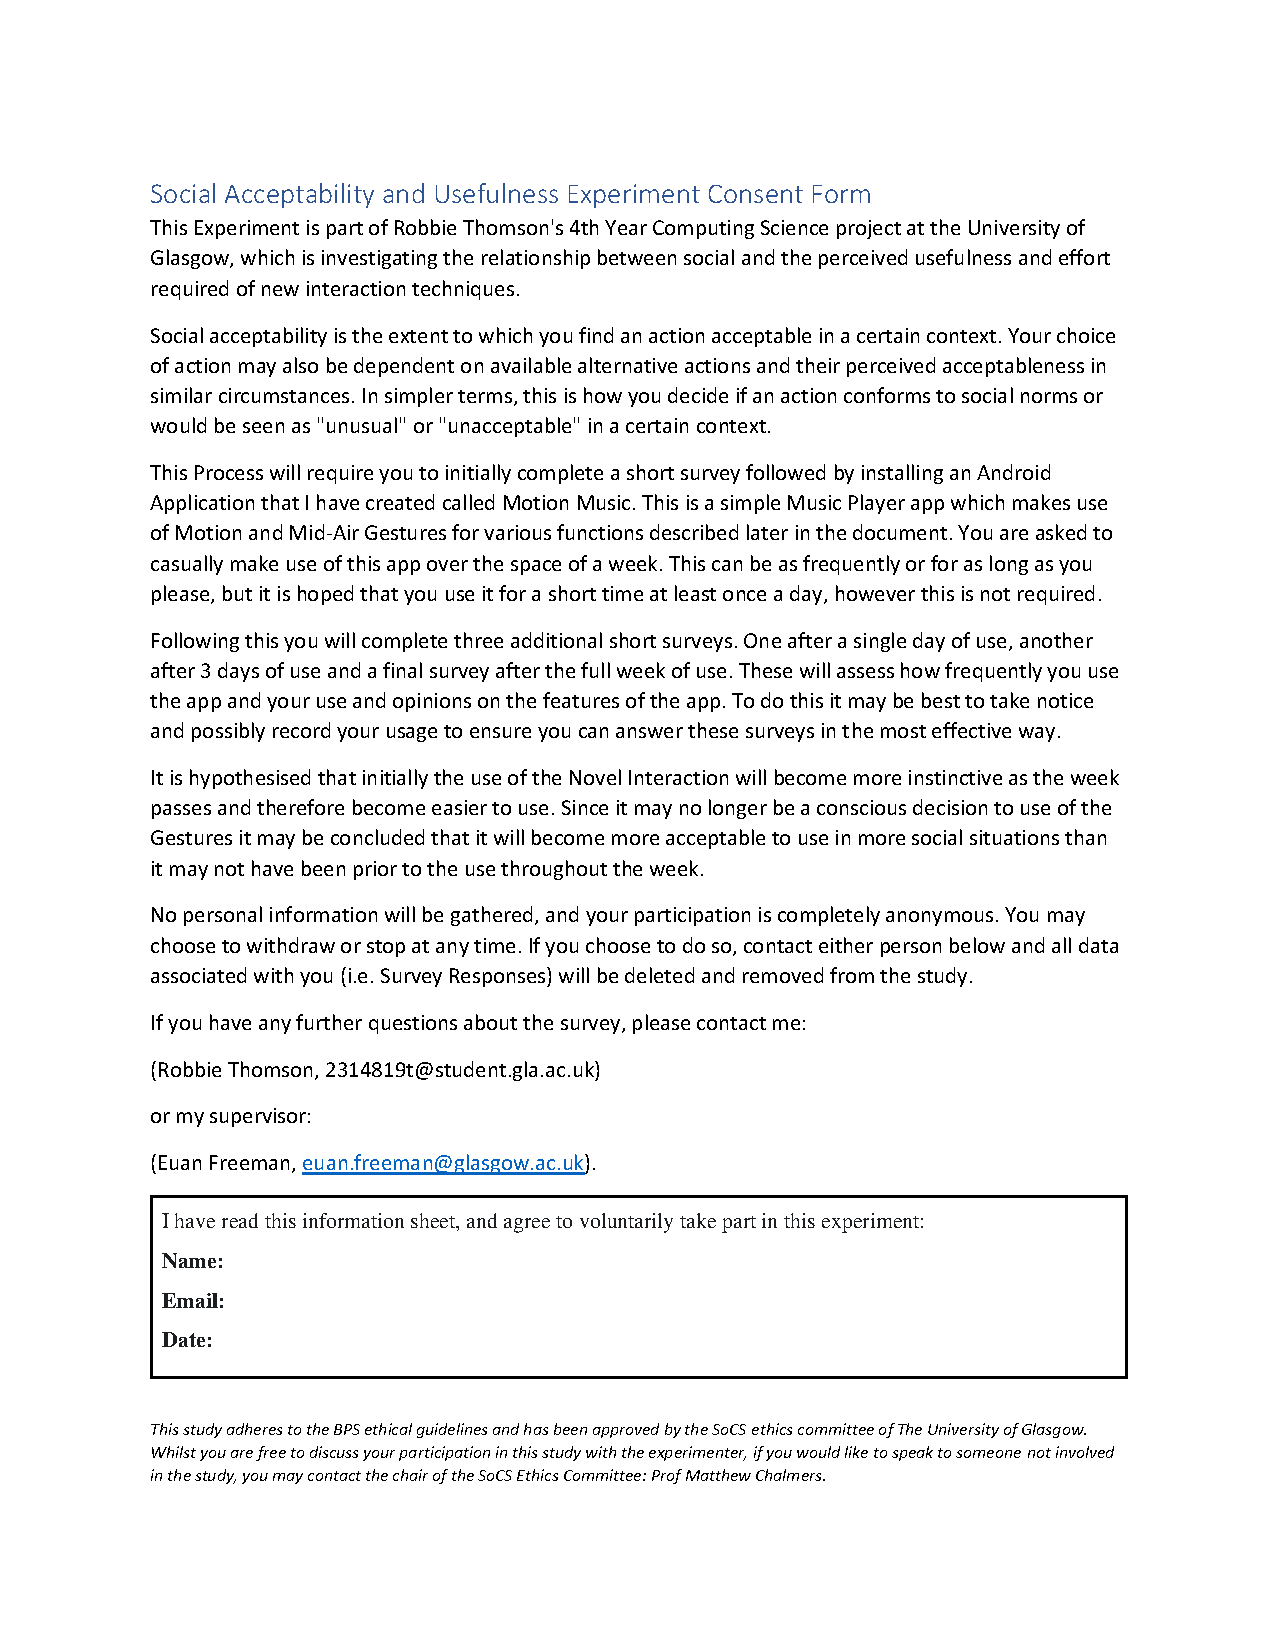
\includegraphics[width=0.9\textwidth]{images/SocialAcceptabilityConsentForm.pdf}
\end{figure}


\chapter{Information Sheet}
Below is the Information Handout supplied to all User Study participants detailing experiment information, installation instructions and Motion Music Usage Details
\begin{figure}[!htb]
    \centering
    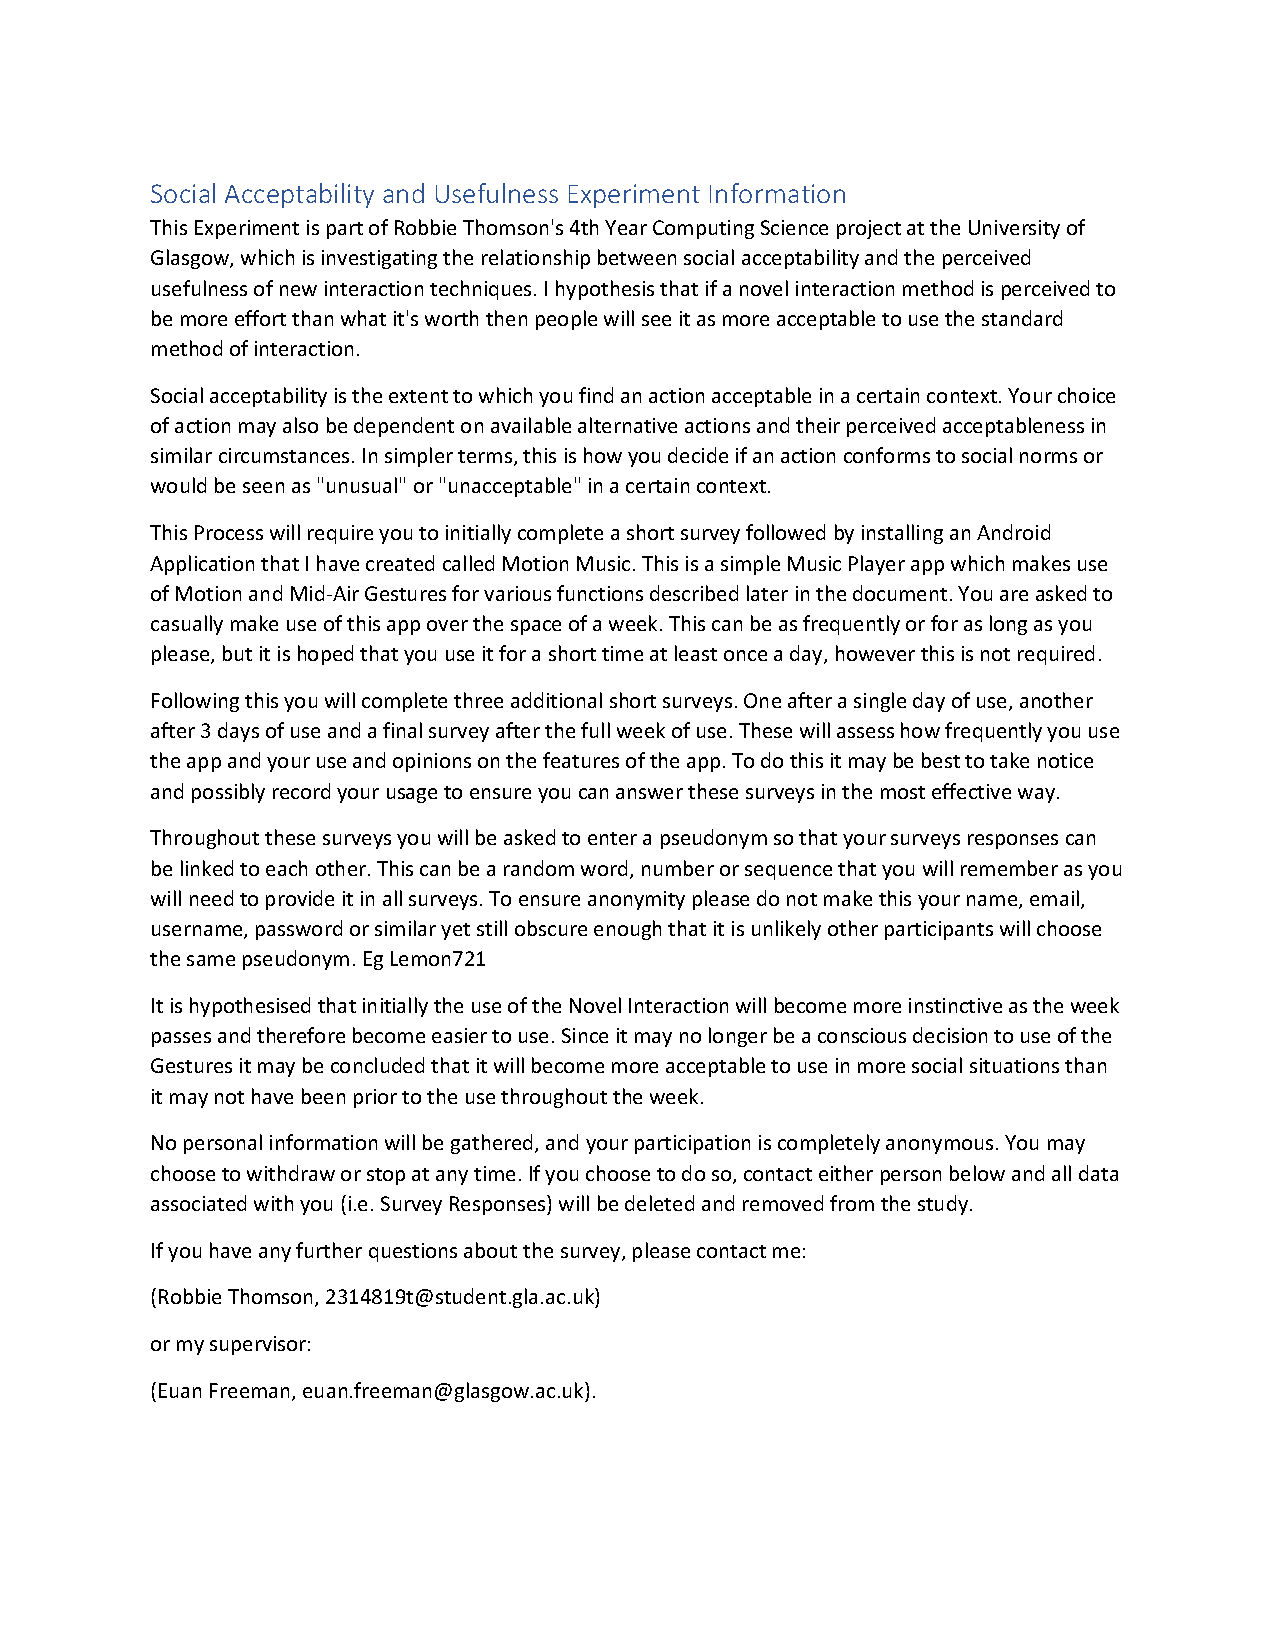
\includegraphics[width=0.9\textwidth]{images/MotionMusicInfoPage.pdf}
\end{figure}

\chapter{Experiment Debrief}
Below is the Experiment Debrief supplied to all User Study participants
\begin{figure}[!htb]
    \centering
    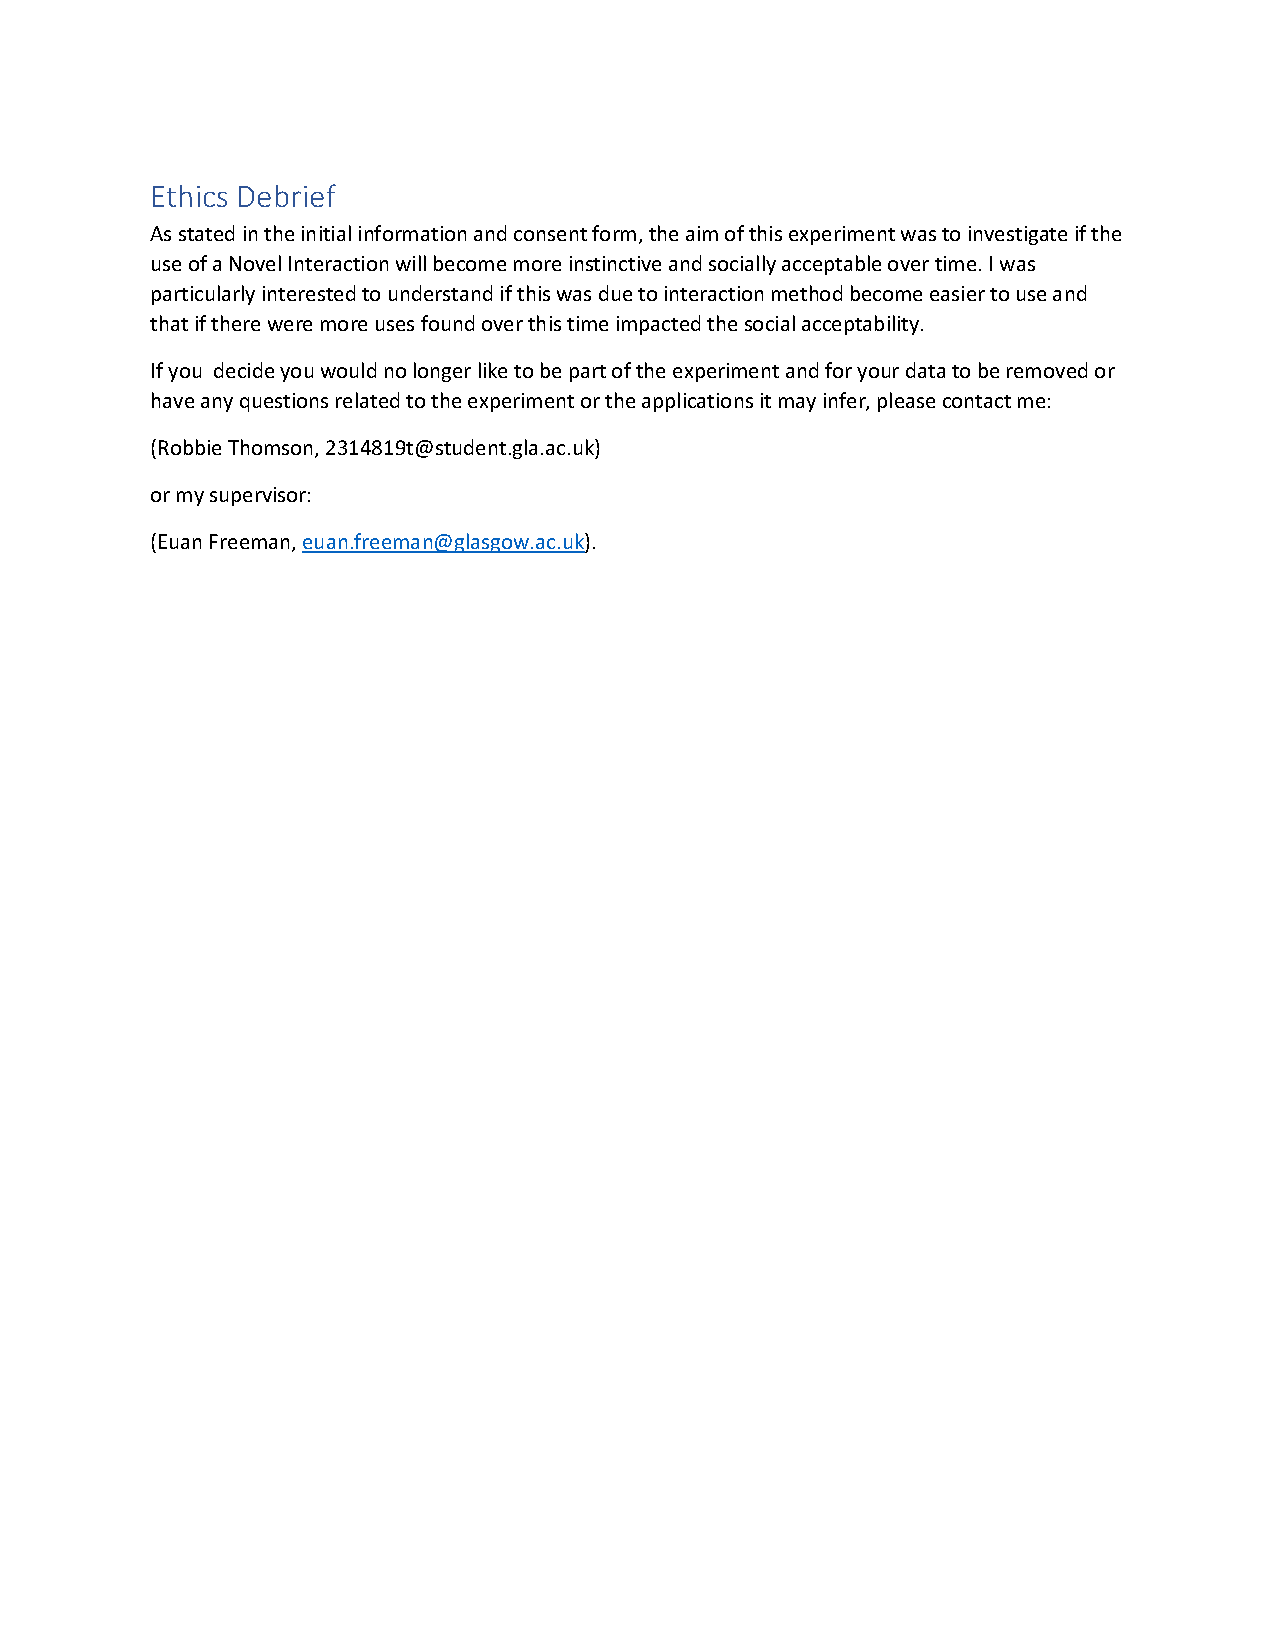
\includegraphics[width=0.9\textwidth]{images/Ethics Debrief.pdf}
\end{figure}


\chapter{References for music used}
\begin{description}
    \item Art Now by Alex (c) copyright 2011 Licensed under a Creative Commons Attribution (3.0) license. Ft: Snowflake
    \item \url{http://dig.ccmixter.org/files/AlexBeroza/30344}
\item
    \item Dj Rkod - Pulse (George Ellinas Remix) by George\_Ellinas (c) copyright 2008 Licensed under a Creative Commons Attribution (3.0) license.
    \item \url{http://dig.ccmixter.org/files/George_Ellinas/14073 }
\item
    \item There's A Better WAY ! by Loveshadow (c) copyright 2011 Licensed under a Creative Commons Attribution (3.0) license. 
    \item \url{http://dig.ccmixter.org/files/Loveshadow/34402 }
\item
    \item Turning Into Normal (What Once Felt Strange) by SackJo22 (c) copyright 2013 Licensed under a Creative Commons Attribution (3.0) license. Ft: Analog by Nature, Haskel (HE31)
    \item \url{http://dig.ccmixter.org/files/SackJo22/43036 Ft: Analog by Nature, Haskel (HE31)}
\end{description}

\end{appendices}

%==================================================================================================================================
%   BIBLIOGRAPHY   

\bibliographystyle{abbrvnat}

\bibliography{l4proj}

\end{document}
